%%% Hlavní soubor. Zde se definují základní parametry a odkazuje se na ostatní části. %%%

%% Verze pro jednostranný tisk:
% Okraje: levý 40mm, pravý 25mm, horní a dolní 25mm
% (ale pozor, LaTeX si sám přidává 1in)
\documentclass[hidelinks,12pt,a4paper]{report}
\setlength\textwidth{145mm}
\setlength\textheight{247mm}
\setlength\oddsidemargin{15mm}
\setlength\evensidemargin{15mm}
\setlength\topmargin{0mm}
\setlength\headsep{0mm}
\setlength\headheight{0mm}
% \openright zařídí, aby následující text začínal na pravé straně knihy
\let\openright=\clearpage

%% Pokud tiskneme oboustranně:
% \documentclass[12pt,a4paper,twoside,openright]{report}
% \setlength\textwidth{145mm}
% \setlength\textheight{247mm}
% \setlength\oddsidemargin{14.2mm}
% \setlength\evensidemargin{0mm}
% \setlength\topmargin{0mm}
% \setlength\headsep{0mm}
% \setlength\headheight{0mm}
% \let\openright=\cleardoublepage

%% Vytváříme PDF/A-2u
\usepackage[a-2u]{pdfx}

%% Přepneme na českou sazbu a fonty Latin Modern
\usepackage[czech]{babel}
\usepackage{lmodern}
\usepackage[T1]{fontenc}
\usepackage{textcomp}

%% Použité kódování znaků: obvykle latin2, cp1250 nebo utf8:
\usepackage[utf8]{inputenc}

%%% Další užitečné balíčky (jsou součástí běžných distribucí LaTeXu)
\usepackage{amsmath}        % rozšíření pro sazbu matematiky
\usepackage{amsfonts}       % matematické fonty
\usepackage{amsthm}         % sazba vět, definic apod.
\usepackage{bbding}         % balíček s nejrůznějšími symboly
			    % (čtverečky, hvězdičky, tužtičky, nůžtičky, ...)
\usepackage{bm}             % tučné symboly (příkaz \bm)
\usepackage{graphicx}       % vkládání obrázků
\usepackage{fancyvrb}       % vylepšené prostředí pro strojové písmo
\usepackage{indentfirst}    % zavede odsazení 1. odstavce kapitoly
\usepackage{natbib}         % zajištuje možnost odkazovat na literaturu
			    % stylem AUTOR (ROK), resp. AUTOR [ČÍSLO]
\usepackage[nottoc]{tocbibind} % zajistí přidání seznamu literatury,
                            % obrázků a tabulek do obsahu
\usepackage{icomma}         % inteligetní čárka v matematickém módu
\usepackage{dcolumn}        % lepší zarovnání sloupců v tabulkách
\usepackage{booktabs}       % lepší vodorovné linky v tabulkách
\usepackage{paralist}       % lepší enumerate a itemize
\usepackage{xcolor}         % barevná sazba
\usepackage{multicol}

\usepackage{rotating}
%\usepackage{fontspec}
\usepackage{tipa}
\usepackage{enumitem}
\usepackage{makecell}
\usepackage{alltt}
\usepackage{refcount}
\usepackage{tabularx}
\usepackage{caption}
\usepackage{pdfpages}       % vložení PDF souboru

%\usepackage{etoolbox}
%\makeatletter
%\patchcmd{\chapter}{\if@openright\cleardoublepage\else\clearpage\fi}{}{}{}
%\makeatother


%%% Údaje o práci

% Název práce v jazyce práce (přesně podle zadání)
%\def\NazevPrace{Reflexe vybraných témat křesťanského myšlení v pojetí Karla Makoně}
\def\NazevPrace{Poselství Karla Makoně}

% Název práce v angličtině
%\def\NazevPraceEN{Reflecting Selected Topics in Christian Thinking in Karel Makoň's Conception}
\def\NazevPraceEN{The Message of Karel Makoň}

% Jméno autora
\def\AutorPrace{RNDr. Jan Oldřich Krůza, Ph.D.}

% Rok odevzdání
\def\RokOdevzdani{2022}

% Název katedry nebo ústavu, kde byla práce oficiálně zadána
% (dle Organizační struktury MFF UK, případně plný název pracoviště mimo MFF)
\def\Katedra{Katedra systematické teologie, teologické etiky a teologické filozofie}
\def\KatedraEN{Department of Systematical Theology, Theological Ethics and Theological Philosophy}

% Jedná se o katedru (department) nebo o ústav (institute)?
\def\TypPracoviste{Katedra}
\def\TypPracovisteEN{Department}

% Vedoucí práce: Jméno a příjmení s~tituly
\def\Vedouci{doc. ThDr. Jiří Vogel, Th.D.}

% Pracoviště vedoucího (opět dle Organizační struktury MFF)
\def\KatedraVedouciho{\Katedra}
\def\KatedraVedoucihoEN{\KatedraEN}

% Studijní program a obor
\def\StudijniProgram{husitská teologie}
\def\StudijniObor{HT NK}

% Nepovinné poděkování (vedoucímu práce, konzultantovi, tomu, kdo
% zapůjčil software, literaturu apod.)
%\def\Podekovani{%
%Děkuji
%}

% Abstrakt (doporučený rozsah cca 80-200 slov; nejedná se o zadání práce)
\def\Abstrakt{%
Karel Makoň (1912-1993) po sobě zanechal rozsáhlé a významné dílo v~psané a
mluvené podobě. Po mystickém zážitku v~koncentračním táboře strávil zbytek
života burcováním k~zasvěcení života hledáním Království Božího. V~desítkách
knih, které napsal, rozvádí návod k~využití pozemského života pro vstup do
vědomého spojení s~Věčností. Hovořil ke skupinkám příznivců, z~čehož se
zachovalo přes tisíc hodin magnetofonových záznamů. Dostupná literatura o něm je
velmi sporadická. Pro šíři jeho hovorů je těžké určit, jaké jsou hlavní body
jeho poselství. Vyskytují se závažné výroky, které v~obměnách opakuje po více
než dvacet let svého auditivně zaznamenaného působení.
}

%%% Hlavní soubor. Zde se definují základní parametry a odkazuje se na ostatní části. %%%

%% Verze pro jednostranný tisk:
% Okraje: levý 40mm, pravý 25mm, horní a dolní 25mm
% (ale pozor, LaTeX si sám přidává 1in)
\documentclass[12pt,a4paper]{report}
\setlength\textwidth{145mm}
\setlength\textheight{247mm}
\setlength\oddsidemargin{15mm}
\setlength\evensidemargin{15mm}
\setlength\topmargin{0mm}
\setlength\headsep{0mm}
\setlength\headheight{0mm}
% \openright zařídí, aby následující text začínal na pravé straně knihy

%% Pokud tiskneme oboustranně:
% \documentclass[12pt,a4paper,twoside,openright]{report}
% \setlength\textwidth{145mm}
% \setlength\textheight{247mm}
% \setlength\oddsidemargin{14.2mm}
% \setlength\evensidemargin{0mm}
% \setlength\topmargin{0mm}
% \setlength\headsep{0mm}
% \setlength\headheight{0mm}
% \let\openright=\cleardoublepage

%% Vytváříme PDF/A-2u
\usepackage[a-2u]{pdfx}

%% Přepneme na českou sazbu a fonty Latin Modern
\usepackage[czech]{babel}
\usepackage{lmodern}
\usepackage[T1]{fontenc}
\usepackage{textcomp}

%% Použité kódování znaků: obvykle latin2, cp1250 nebo utf8:
\usepackage[utf8]{inputenc}

%%% Další užitečné balíčky (jsou součástí běžných distribucí LaTeXu)
% Abstrakt (doporučený rozsah cca 80-200 slov; nejedná se o zadání práce)


%% Balíček hyperref, kterým jdou vyrábět klikací odkazy v PDF,
%% ale hlavně ho používáme k uložení metadat do PDF (včetně obsahu).
%% Většinu nastavítek přednastaví balíček pdfx.
\hypersetup{unicode}
\hypersetup{breaklinks=true}

%% Definice různých užitečných maker (viz popis uvnitř souboru)

\begin{document}

\chapter*{Iterative Improving of Transcribed Speech Recordings Exploiting Listener's Feedback}

\section*{Abstract}

\thispagestyle{empty}

This Ph.D. thesis deals with making a corpus of audio
recordings of a single speaker accessible to wide public and interested community.

The work has been motivated by the existence of a set of perishing recordings
of the Czech philosopher Karel Makoň on magnetophone tapes. The aim is to conserve
the material for future generations and making it accessible using
digital technologies, in particular publishing the recordings online
and enabling the users to search through them.

The thesis introduces the creation of a system for transcribing a large set of
speech recordings employing a lay community. The solution designed is based on
obtaining a baseline low-quality transcription by means of automated speech
recognition and developing an application that allows for collecting corrections
of the automatic transcription in a fashion that makes it usable as training
data for further improvement of said transcription.

The spoken corpus itself is described. The
author and his works, topics covered in the talks, the process of recording
and digitization as well as the gained transcription are introduced.
Next, the development of a system for automated transcription of
the corpus, from collecting data, to acoustic and language modeling, various experiments
undertaken and evaluation are presented. Then, the web application for gathering
manual transcript corrections is described.
Differences to other settings, design and implementation details, a way to
compensate high demand for transcription quality and low demand for worker
expertise, as well as an evaluation of the system's performance after eight
years of operation are covered.

\end{document}


% 3 až 5 klíčových slov (doporučeno), každé uzavřeno ve složených závorkách
\def\KlicovaSlova{%
{Karel Makoň}, {křesťanská mystika}, {systematická teologie}, {extrakce klíčových slov}
}
\def\KlicovaSlovaEN{%
{Karel Makoň}, {Christian Mysticism}, {Systematical Theology}, {Keyword Extraction}
}

%% Balíček hyperref, kterým jdou vyrábět klikací odkazy v PDF,
%% ale hlavně ho používáme k uložení metadat do PDF (včetně obsahu).
%% Většinu nastavítek přednastaví balíček pdfx.
\hypersetup{unicode}
\hypersetup{breaklinks=true}

%% Definice různých užitečných maker (viz popis uvnitř souboru)
\include{makra}

%% Titulní strana a různé povinné informační strany
\begin{document}
%%% Titulní strana práce a další povinné informační strany

%%% Titulní strana práce

\pagestyle{empty}
\hypersetup{pageanchor=false}

\begin{center}

{\bf\Large UNIVERZITA KARLOVA}

\vfill

{\Large HUSITSKÁ TEOLOGICKÁ FAKULTA}

\vfill

\centerline{\mbox{\includegraphics[width=66mm]{rc/logo-htf.jpg}}}

\vfill

{\bfseries\NazevPrace}

\vfill

{\bfseries\NazevPraceEN}

\vfill

Seminární práce

\vspace{15mm}

\begin{multicols}{2}
Vedoucí práce:\\
\Vedouci\\
\columnbreak
Autor:\\
\AutorPrace\\
\end{multicols}

\vfill

% Zde doplňte rok
Praha \RokOdevzdani

\end{center}

\newpage

%%% Strana s čestným prohlášením k disertační práci

\openright
\hypersetup{pageanchor=true}
\pagestyle{plain}
\pagenumbering{roman}
\vglue 0pt plus 1fill

\noindent
Prohlašuji, že jsem tuto seminární práci vypracoval samostatně a výhradně
s~použitím citovaných pramenů, literatury a dalších odborných zdrojů.

\medskip\noindent
Beru na~vědomí, že se na moji práci vztahují práva a povinnosti vyplývající
ze zákona č. 121/2000 Sb., autorského zákona v~platném znění, zejména skutečnost,
že Univerzita Karlova má právo na~uzavření licenční smlouvy o~užití této
práce jako školního díla podle §60 odst. 1 autorského zákona.

\vspace{10mm}

\hbox{\hbox to 0.5\hsize{%
%V \hbox to 6em{\dotfill} dne \hbox to 6em{\dotfill}
V Praze dne \today
\hss}\hbox to 0.5\hsize{\dotfill\quad}}
\smallskip
\hbox{\hbox to 0.5\hsize{}\hbox to 0.5\hsize{\hfil Podpis autora\hfil}}

\vspace{20mm}
\newpage

%%% Poděkování

\openright

\noindent
%\Podekovani

%\newpage

%%% Povinná informační strana disertační práce

%\openright

%\vbox to 0.5\vsize{
%\setlength\parindent{0mm}
%\setlength\parskip{5mm}

%{\bf Abstrakt:\\}
%\Abstrakt

%{\bf Klíčová slova:\\}
%\KlicovaSlova

%\vfill

%{\bf Abstract:\\}
%\AbstraktEN

%{\bf Keywords:\\}
%\KlicovaSlovaEN

%\vss}

\newpage



\openright


%%% Strana s automaticky generovaným obsahem disertační práce

\tableofcontents

\newpage
\pagenumbering{arabic}
\setcounter{page}{1}
%%% Jednotlivé kapitoly práce jsou pro přehlednost uloženy v samostatných souborech

\chapter{Úvod}
\label{kap:uvod}

Není jistě zvykem začínat práci o významné osobnosti vlastním příběhem.
Dopouštím se toho v~naději, že tím vrhnu trochu světla na to, co vlastně Karel
Makoň přinesl.

Od věku dospívání jsem četl dostupnou duchovní a ezoterickou literaturu. Zaujala
mě tantra, obzvláště v~podání Andrého van Lysebetha\cite{LysebethTantra}, potom
ezoterika, jak ji představoval Thorwald Dethlefsen\cite{DethlefsenOsud}. Ten mě
motivoval k~tomu, abych hledal poznání nejen vědecky, objektivně ve vnějším
světě, ale i ezotericky, nesdělitelně, ve vnitřním světě. 

\chapter{Osobnost Karla Makoně}

\section{Životopis}

Pokusím se přiblížit, co za člověka Karel Makoň byl tím, že převyprávím jeho
život podle toho, jak a s~jakými důrazy ho podává on sám. Je to příběh plný
zázraků, což odpovídá tomu, že Makoň na svém životě demonstruje působení
zázračného tažení Božího. Nic mu to ale aspoň v~mých očích neubírá na
pravdivosti.

Stať o Makoňově životě čerpá z~jeho knihy Umění žít a ze záznamů nahrávek.

\subsection{Poznávání správného}

Karel Makoň se narodil 12.12.1912 v~Ošelíně u Plzně. Jeho otec osm měsíců na
to zemřel na tuberkulózu a Karel sám dostal zánět do levého ramene. Ten dospěl
do takového stádia, kdy lékař doporučil amputaci ruky. Matka toto odmítla a tak
započala první fáze Makoňovy duchovní formace. Rameno bylo nutno operovat.
Jelikož se ještě nepoužívala transfúze, musela se operace provádět na
několikrát, protože jinak by dítě vykrvácelo. A kvůli Makoňově útlému věku a
stavu tehdejší anesteziologie musely operace probíhat za vědomí. Dítě bylo
vystaveno takové bolesti, že se naučilo vystupovat z~těla. Toto se podle
Makoňových slov opakovalo čtrnáctkrát, což malého Karla Makoně nezvratně
změnilo.

Ve stavech mimo tělo, kdy necítil bolest, se setkával s~něčím, co nazývá
,,žlutým světlem``.  Důsledkem bylo, že dítě začalo samovolně rozlišovat, co je
správné, a byl vnitřně puzen správné následovat. Správné od nesprávného dokázal
rozpoznat, ale neměl schopnost správné řešení situace sám vymyslet. Důvěřoval
matce a tak ji častoval otázkami, jak se má zachovat. Mnohokrát pak její návrh
odmítl s~tím, že tohle dělat nebude a trval na tom, že musí dostat jiný. Jeho
matce se zdálo, že dítě si svévolně vybírá a matku trápí.

V~období raného dětství vyčníval Karel Makoň nejen puzením ke správnému, ale
také intenzivním stykem se zvířaty. Aby se operované rameno neporanilo, měl
Karel Makoň zapovězeno hrát si s~jinými dětmi. Trávil proto svůj volný čas
v~předškolním věku téměř výhradně o samotě se zvířaty, obzvláště s~husami.
Naučil se rozumět jejich řeči a ony ho přijali mezi sebe jako jednoho z~nich.

Makoň poznal, že husy ve stavu spánku nejsou nečinné, nýbrž žijí intenzivním
životem na jiné úrovni. Vzaly ho oďobáváním na správných místech s~sebou a on
s~nimi prožíval ,,stav zvířecího ráje``, kde bylo přítomno celé stádo, ale
nikoliv v~tělech, nýbrž bez nich. Prožívali pospolitost, viděli na sobě, jaké
mají neduhy a co je potřeba k~jejich překonání.

Poznání skutečného zvířecího ráje, ke kterému nemá běžný člověk přístup, a
puzení vyhnout se nesprávnému, vedly Karla Makoně k~pevnému rozhodnutí vystříhat
se veškerého ,,pohlavního života``, jak sexuální aktivitu konzistentně nazývá.

Jeho matka a obzvláště babička Karla Makoně vedly ke zbožnému katolickému
životu. Musel se pravidelně modlit a chodit do kostela. Vysvětlovaly mu to tak,
že nebude-li toho činit, přijde do pekla, zatímco když bude, dojde do nebe, kde
se bude věčně dívat na Boží tvář. Makoňovo inspirované rozpoznání správného a
nesprávného mu neomylně radilo, že tohle správné není a tak nevěřil, do nebe se
dostat nechtěl, protože takto popsané mu připadalo jako ukrutná nuda, a modlitby
prováděl jen matce a babičce kvůli, neboť rozpoznával jako správné řídit se
jejich vůlí.

Ve škole prožíval Karel Makoň těžké loučení se zvířecím světem a sžívání s~tím
lidským. Poznával ale jak v~matce tak v~učitelích autority, takže se převychovat
nechal. Vedlo to nakonec k~tomu, že Karel Makoň si v~životě vytvořil jedinou
skutečnou lásku, a tou byly přírodní vědy. Toužil stát se přírodovědcem víc než
cokoliv jiného. Když ho pak rodinná finanční situace donutila se tohoto snu
vzdát, ztratil svoji jedinou lásku a s~tím jakoby sama sebe.
Tímto dospěl do druhého zlomu po operacích ramene.

\subsection{Modlitba za lásku}

Makoň byl nucen studovat ekonomii a aby aspoň nějak ukojil touhu po přírodních
vědách, chodil si číst přírodovědné knihy do knihovny. Při jedné takové
příležitosti namátkou otevřel knihu a oči mu padly na větu, která ho uchvátila a
strhla do prvního vytržení. Stálo tam \textit{,,tento život je mostem do
věčnosti``}.

Tento zdánlivě banální zážitek poskytl Makoňovi niterné setkání se svojí věčnou
podstatou, ovšem jen chvilkově. Tehdy absolutně ztratil zájem o všechny světské
záležitosti. Matka ho musela několik dní nutit do jídla a spánku, studiu se
věnoval s~extrémní nechutí a jen kvůli svým blízkým. Jediným jeho zájmem se
stalo spojení s~Věčností, které zakusil v~knihovně.

Tehdy si vzpomněl na svoji katolickou výchovu a obrátil se na kněze s~prosbou o
generální zpověď. Jaký byl knězův údiv, když ho Makoň žádal o rozhřešení za to,
že nežil dosud jen pro Boha! A o kolik větší byl ještě jeho údiv, když při
dalším setkání Makoň tvrdil, že nezhřešil. Konsternovanému knězi to vysvětlil
tak, že nemůže hřešit, i kdyby chtěl, protože pociťuje přítomnost Boží a ta mu
žádný hřích nedovolí.

Vytržení, nebo jak je sám nazývá \textit{,,extaze``} zažíval opakovaně. Pokaždé
v~nich zažíval jistotu vlastního zániku a s~hrůzou utekl a pokaždé si pak
předsevzal, že příště již neuteče. Stanovil si nejpřísnější řeholi, jaká ho
napadla, a modlil se bez ustání výhradně za to, aby dokázal Boha více milovat,
neboť cítil, že k~Němu chová lásku zcela neadekvátní Boží vznešenosti. Ba
pociťoval to tak, že vlastně vůbec žádné lásky není sám schopen.

Toto trvalo devět let a vyústilo do dalšího, zdaleka nejzávažnějšího zlomu
v~Makoňově životě.

\subsection{Koncentrační tábor}

Datum sedmnáctého listopadu máme spojeno se Sametovou revolucí, kde výraznou
roli hráli demonstrující studenti. Je pozoruhodné, že v~týž den roku 1939, tedy
přesně půl století před tím, byly nacisty uzavřeny české vysoké školy a studenti
deportováni k~likvidaci. Toho se stal obětí i Karel Makoň. Je trochu ku podivu,
že byl i on deportován, neboť při zásahu nacistů nebyl ve škole. Došel již do
prázdné budovy později a odvedené spolužáky sám vyhledal a přihlásil se k~nim.
Poté dokonce vyvolávali jeho jméno, jako jednoho z~těch, kteří měli být
propuštěni, neboť měl už fakticky studium za sebou. Dostal ovšem před tím ránu
pažbou do hlavy a dočasně ztratil sluch, takže nevěděl, že je vyvoláván.

V~koncentračním táboře nastalo pro Makoně naprosté peklo. Snad k~tomu přispěla
zakrnělá ruka\footnote{Toto je domněnka autora.}, že Makoň schytával bití,
šikanu a ústrky více než ostatní spoluvězni. Ti se nejednou podivili, že
kdykoliv se rozdávaly rány, Makoň jako by se tam zákonitě připletl a schytal
ještě víc.

Snad ještě horší než faktické strádání násilím, hladem, nečistotou a vůbec
podmínkami k~živoření byl pro Makoně fakt, že po devíti letech usilovné modlitby
za větší lásku k~Bohu, absolutní čistoty a věrnosti, s~ním mají duchovně
zakrnělí lidé právo nakládat jako s~kusem hadru. Cítil se Bohem opuštěn a
zrazen. A dodává, že kdykoliv si toto pomyslel, hned tu byl kopanec nebo políček
od dozorce.

Tragická epizoda vyvrcholila 21. listopadu 1939 po čtyřech dnech krutého utrpení. Vězňové
v~koncentračním táboře měli zapovězeno sledovat, jak některý z~jejich spoluvězňů
je vražděn nacistou. Makoně ovšem jeden z~Němců právě při tomto přistihl. Právě
dobíjel jednoho vězně a vyzval Makoně, aby zůstal na místě, že hned po něm je na
řadě on. Vyzbrojen svými předchozími zážitky a devítiletou disciplínou, dokázal
Karel Makoň v~gestapákovi\footnote{Zda se jednalo skutečně o příslušníka Gestapa
mi není známo, ale jako o gestapákovi nebo o esesákovi se Makoň o dotyčném často
zmiňuje.} nevidět zrůdu, ale posla Božího. Klidně, bez slovních deklarací,
složil život do Božích rukou. Gestapák se už napřahoval k~zasazení rány, když
v~tom hrůzou zbledl a obrátil se na útěk.

Karel Makoň v~této chvíli mystické smrti, kdy vnitřně zemřel ještě než zemřel
fyzicky, podle svých slov obdržel najednou poznání významu celé situace. Poznal,
proč je v~koncentráku, proč tam je každý z~ostatních, za jakých podmínek se
odtamtud dostane, a především obdržel poznání celé symboliky biblického textu,
katolické tradice i jiných svatých písem.

Od tohoto momentu se Makoň vyvázal z~veškerého utrpení. Jedl i pil dále stejně
jako ostatní, ale příděly mu bohatě stačily. Zažíval naprostou svobodu.
Procházel volně bezi baráky, hlídky ho nikdy nespatřily. Všem svým spoluvězňův
kázal slovo Boží a osvětloval jim, jak se i oni mohou z~utrpení vyvázat.

\subsection{Život v~Boží přítomnosti}

Ve vydávání svědectví o tom, že lze dosáhnout vědomého spojení s~Bohem, vytrval
Makoň i po propuštění z~koncentračního tábora. Zasvětil celý zbytek života tomu,
aby svoje poznání předal dál a aby pomohl ostatním lidem k~tomu, aby i oni
naplnili smysl života, ovšem bez tak těžkých krizí, jaké sám zažíval. Napsal
dvacet sedm knih a dvacet osm jich přeloži a komentoval. Všechny jsou dostupné
na internetové stránce \url{makon.cz}.

Krom psaní pravidelně přednášel v~úzkém kruhu přátel na~různých místech
Československa. Měl skupinku posluchačů především ve Zlíně, v Plzni a v Praze.
Tyto spontánní přednášky, které se odehrávaly většinou u některého účastníka
doma nebo na několikadenním výjezdu, někteří účastníci nahrávali na
magnetofonové pásky. Z~toho vznikl archiv více než tisíce hodin záznamu. Jeho
zpracování a zpřístupnění je tématem mojí informatické disertační
práce\cite{kruuza2021iterativni}. Nahrávky jsou dostupné na adrese
\url{radio.makon.cz}.

Občanským zaměstnáním byl Makoň středoškolským učitelem, z~čehož také plyne
tradice mezi jeho příznivci, nazývat ho profesorem. Oženil se a měl tři děti.
%TODO: kdy zemřela manželka?
Zemřel 24. října 1993, rok po svojí poslední přednášce. Jeho život byl protkán
zázračnými událostmi, z~nichž některé si získaly punc významnosti. Ty jsou
sepsány v~knížce Mozaika mystického života Karla Makoně\cite{mozaika}, kterou na
jeho památku jeho následovníci po jeho smrti sepsali.

\section{Anekdoty}

Příběh o tom, jak Karel Makoň překonal smrt v~koncentračním táboře a jak byl na
tuto mezní událost připravován, nám přibližuje, jak se z~něho stal člověk,
kterým byl po celý zbytek života. Jak ale s~touto hřivnou hospodařil? Jaký byl
jako člověk? Na tuto otázku mohu sám odpovědět jen těžko, sám Makoně nezaživ.

V~jeho řeči rozpoznávám přirozenou autoritu a humor. Jeho žáci, které znám, ho
často citují a je znát, že pro ně byl nezpochybnitelnou autoritou a že ho
nesmírně milovali. Mnohdy se vyprávění koncentruje na zázračné události, který
ten který svědek s~Makoněm zažil. Jeden z~výrazných Makoňových žáků svědčí o
tom, že s~Makoněm bylo veselo. Říká, že se někdy smáli tak, až ho prosil, ať už
té legrace nechá, jinak že snad tolik veselí ani nevydrží. Tomu nasvědčuje i
fakt, že Makoň byl alergický na takzvané \textit{,,smutné svaté``}.

\subsection{Záhrobí}

Karel Makoň svoji manželku přežil. Na sklonku života trpěla bolestmi a Makoň ji
naučil dechovými technikami opouštět tělo. Když tedy přešla práh smrti, měla již
za sebou jistý trénink a na onom světě žila poněkud uvědomělejším životem. Makoň
s~ní pak vedl velmi bohatou a dlouhodobou komunikaci, která mu zprostředkovala
kromobyčejně detailní informace o záhrobním životě.

%Koluje legenda, že ve dvanáct hodin a
%dvanáct minut, ovšem sám Karel Makoň zmiňuje v~Umění žít\cite{KaMaUZ}, bylo to
%podle záznamu jeho otce v jednu hodinu a devatenáct minut v noci.

\chapter{Kontext Makoňova působení}

\section{Makoňova doba}

Karel Makoň prožil skoro celé dvacáté století, takže jeho doba byla velmi
různorodá. Narodil se ještě v~Rakousku-Uhersku, čemuž odpovídá jeho tradiční
katolická výchova. Do základní školy chodil v~čerstvě vzniklém
Československu, takže zakusil ještě školství v tereziánském duchu. Budeme-li u
něho rozeznávat tři hlavní období:
\begin{enumerate}
\item{puzení ke správnému, tj. od operací ramene do první extáze (1930),}
\item{modlitbu za lásku k~Bohu, tj. od první extáze do mystické smrti
v~koncentračním táboře (1939) a}
\item{aktivní tvorbu, tj. od propuštění z~KZ do smrti,}
\end{enumerate}
zkonstatujeme, že první období -- dětství prožíval v~době první světové války a
rané první republiky. Druhé období prožíval v~době pozdní první republiky a
během prvních dnů protektorátu. Za druhé světové války ho zastihl nejvyznamnější
formující prožitek v~koncentračním táboře. Většinu války i další události už pak
prožil ve stavu praktické odpoutanosti od vnějších poměrů.

Je zřejmé, že vnější okolnosti hrály v~jeho formování do roku 1939 zásadní roli:
\begin{itemize}
\item{stav medicíny, který umožnil operace, ale neumožnil anestezii ani
transfúzi,}
\item{prostý venkovský život, který umožňoval strávit většinu raného dětství
s~husami,}
\item{trvající vliv rakousko-uherského katolicismu,}
\item{rostoucí popularita okultismu a mystiky}
\item{a konečně nacistický teror vedoucí k~prožitku mystické smrti.}
\end{itemize}

Makoňovo zaměření nebylo do záležitostí tohoto světa a jeho fundamentální
poselství je nadčasové, nezávislé na poměrech. Přesto by bylo mylné se domnívat,
že vnější okolnosti po roce 1939 Makoně neovlivňovaly. Ovlivňovaly, a to
zásadně, byť se ho nemusely niterně dotýkat. Jednak sice jeho zaměření nemuselo
být do záležitostí tohoto světa, ale lidské duše, kterým chtěl dopomoci ke
spáse, se v~tomto světě nacházely, a ve světě viděl ke spáse nezbytný
prostředek,\rref{78-05A-Kaly}{26:29} jednak se za jeho působení výrazně změnily podmínky pro šíření
náboženských nauk.\cite{nevspor2007vceska} Po skončení druhé světové války v~Československu, na krátko
zase svobodném, mohl Makoň svoje svědectví šířit jako středoškolský učitel
otevřeně i mezi žáky a samozřejmě mezi známými. Když pak došlo v~roce 1948
k~bolševickému puči, stalo se postupně náboženství i duchovno obecně
tabuizovaným oborem.\cite{kaplan1993stat} Makoň v~souladu se svojí naukou, že nemá smysl plýtvat
silami na boj s~režimem -- podobně jako sv. Josef utekl od Heroda, místo aby
s~ním bojoval -- se stáhl do ústraní. Působil dál, ale v~uzavřených kruzích.

Dočasné rozvolnění v~šedesátých letech ani pád socialistického bloku v~roce 1989
tento Makoňův styl nezměnily. Na veřejnost ani do médií se nijak nehrnul a
pokračoval ve svém psaní a přednášení a celkovém nenápadném působení do konce
života.

\section{Předchůdci}

Makoň se sám řadí do tradice křesťanské mystiky.\footnote{Viz spis Mystika I,
str. 14, kde autor praví: \textit{,,Definujme mystiku prostě
jako hledání spojení s~Bohem už v~tomto životě zde na zemi a
podrobování celého života tj. celého myšlení, konání a cítění
tomuto cíli.``} Tomu Makoň zasvětil celé dílo.} Bylo by tedy vhodné zařadit ho
do kontextu této tradice. Odvolává se na mnoho autorů. Dá se ale říci, že jen
dva jsou podle všech kritérií jeho předchůdci, a těmi jsou Mistr Eckhart a svatá
Terezie z~Avily.

Makoň mezi autory, na které navazuje, rozeznává dvě kategorie:
\begin{enumerate}
\item{ty, kteří prožili mystickou smrt a}
\item{ty, kteří mystickou smrt neprožili.}
\end{enumerate}
Nechci hodnotit, nakolik je to legitimní rozdělení a nakolik bylo
z~Makoňovy strany přesné. Jednak se k~tomu necítím povolán a jednak jsem coby
Makoňův příznivce pozitivně předpojat. Nejde mi zde však o nějaké objektivní
vymezení toho, kdo jaký byl, ale o to, ke komu se jakým způsobem Makoň hlásí.
Jeho předchůdce tedy míním v~tom smyslu, koho by za svého předchůdce sám asi
považoval.

Z~těch, kteří se křesťanské mystice věnovali, ale kteří podle Makoně smrtí na
kříži neprošli, jmenuje např. Molinose\rref{80-11A}{32:35} nebo Bernarda z~Clairvaux, kterého rád
nazývá kvůli podílu na křížové výpravě prasákem.\rref{91-05A}{12:45} Odkazuje se naopak na některé
světce, které skutečně za svaté (a tedy prošedší mystickou smrtí) považuje, ovšem
kteří se nezabývali křesťanskou mystikou tak vyhraněně, aby mohli s~ním být
postaveni do řady. Z~nich jmenujme např. svatého Antonína
Velikého\rref{83-10}{58:10} nebo svatou
Anežku Českou.\rref{kotouc-S01-a}{18:13} V~podobné kategorii by mohli být Makoňovy vzory z~nekřesťanských
kultur: Lao C',\rref{87-03}{44:02} Šrí Aurobindo Ghóš,\footnote{Mystika II,
svazek Ghos I, str. 21} Ramakrišna.\rref{84-09A-84-03-20}{43:56} Lze zmínit i Makoňovy vzory
starozákonní: Například proroka Eliáše\rref{90-05A}{12:41} a duchovní vůdce
Izreale považuje za lidi prošedší také smrtí na kříži. Ne tak ovšem již pisatele
Starého zákona.\rref{82-03}{01:36:11}

Dva stěžejní Makoňovi předchůdci, kterým připisuje nemenší úroveň poznání, než jakou
rozpoznával u sebe, a kteří se také věnují křesťanské mystice, se samozřejmě od
Makoně podstatně odlišují. Jednak oba dva měli už za svého života značný vliv a
pozornost,\cite{hackett2012companion}\cite{britannicaTeresa} jednak je nauka každého z~nich posazená do zcela jiné doby. Jejich
porovnání by bylo na samostatné práce, ale zmiňme aspoň ty nejpatrnější rozdíly:
Většina dochovaných Eckhartových děl jsou kázání, takže zcela jiný žánr, než do
jakého můžeme zařadit Makoňovo dílo. Eckhartova řeč je také mnohem více
postavena na šokujících a těžko srozumitelných výrocích, které mají vytrhnout
posluchačovu mysl a unést ji k~Bohu,\cite{landauer1978eckhart} zatímco Makoň píše systematicky a, mám-li
parafrázovat jeho vlastní slova, píše tak, aby přesvědčil rozum, že se má dát do služeb
Božích. Svatá Terezie z~Avily naproti tomu musela harmonovat, aspoň do jisté
míry, s~tehdejší církevní doktrínou.\cite{eire2019life}

\section{Současníci}

Kategorii Makoňových současníků můžeme vymezit bez ohledu na jeho vlastní postoj
vůči nim, i když samozřejmě Makoňovy postoje jsou jedním z~hlavních kritérií,
podle kterých můžeme rozhodnout, kterého z~jeho současníků máme jmenovat. Makoň
začínal působit v~době, kdy česká mystika byla prakticky definovaná osobností
Karla Weinfurtera.\cite{sanitrak2006dejiny1} Je proto logické, že se na něj
často odvolává, že v~jejich učeních nalezneme mnohou shodu, i že se vůči
Weinfurterovi Makoň vymezuje. Vymezení je především vůči praktikám jeho
následovatelů a podobnosti nalezneme velmi hojně a netřeba pro ně chodit
daleko. Hned v~úvodu k~Ohnivému keři\cite{weinfurter1923ohnivy} nalézáme
myšlenku, že je potřeba uvést na pravou míru chybně interpretované křesťanské
učení. Makoň, stejně jako Weinfurter, pokládá jógu za ekvivalent mystické cesty,
odvolává se na rádža jógu, Paula Bruntona atd.

Druhým výrazným Makoňovým současníkem je Eduard Tomáš. Tomáš byl starší než
Makoň, ale zemřel později (*1908 \textdagger2002). I jejich nauky se překrývají
v~mnoha bodech, a to i těch hlavních: Není trvalého štěstí v~žádném předmětu
tohoto světa; naše skutečná podstata je božská; atd.

Hlavní rozdíly oproti Weinfurterovi i Tomášovi vidím dva shodné: Oba byli
exponovaní na veřejnosti, zatímco Makoň nikoliv, to za prvé. Za druhé, Makoň
sice nezapadá do žádné církevní doktríny, ale je vyhraněně křesťanský.
Zdůrazňuje, že jediným mistrem je Ježíš Kristus. Jediným vzorem hodným
následování je Ježíš Kristus. Makoň se vlastně snaží přivést lidi k~tomu, aby
plodně následovali Ježíšova příkladu. V~tomto se jak od Weinfurtera, pro kterého
je podstatná mystická zkušenost, i od Tomáše, který klade důraz na Absolutno,
liší. Pro Tomáše je království nebeské stav štěstí a klidu.\footnote{Paměti
mystika 1. díl, od 02:52 \href{https://youtu.be/4nVY5RvOjs4?t=172}{youtu.be/4nVY5RvOjs4?t=172}.} Pro Makoně je to
podřízení vlastní vůle vůli Boží. A z~mého hlediska to Makoně staví na pevnější
půdu.

\section{Shrnutí}

Většina velkých osobností dojde svého zařazení a hodnocení až s~jistým odstupem.
Jak dlouho to bude trvat u Karla Makoně, nelze předvídat. Některé osobnosti,
jako svatá Hildegarda z~Bingen, došly širšího uznání až skoro po mnoha
staletích.\footnote{Srovnej počty publikací o sv. Hildegardě podle roku jejich
vzniku.} Jiné možná nikdy, což nevíme, protože kdybychom věděli, nebyly by
neznámé. Dával jsem Karla Makoně do srovnání s~osobnostmi, od kterých všech se
odlišoval tím, že nedospěl popularity. Je to logické, neboť ho nemůžeme
srovnávat s~neznámými osobnostmi, opět protože o nich nevíme. Navíc je tato
práce psána z~pohledu člověka, který v~Makoňovi velkou a vyčnívající osobnost
spatřuje.

Je jasné, že vliv okolí na Makoňovu tvorbu nelze zhodnotit: Každá událost je
organicky zařazena do svého prostředí a v~jiných podmínkách ji zkrátka nelze
zkoumat. Snad se však podařilo nastínit aspoň nejhrubší souvislosti, bez jejichž
povědomí nelze Makoňovo dílo hodnotit ani mu rozumět.

\chapter{Literatura o Karlu Makoňovi}

bakalářka

mozaika

dingir

web

moje

\chapter{Vybraná témata v~pojetí Karla Makoně}

Při opakovaném poslechu Makoňových hovorů si všímám, že určitá sdělení se
neustále vracejí a ačkoliv je pokaždé trochu jiné, ve stěžejních bodech zůstává
stále totéž. Mohu uvést několik příkladů takových sdělení, se kterými se
opakovaně u Karla Makoně setkávám:

\begin{enumerate}
  \item{
      Cesta k Bohu se dělí na fáze. Podle toho, kde se nacházím, platí pro mě
      jiné zákonitosti.  Mezi fázemi jsou ostré předěly.
  }
  \item{
      Pro spojení s Bohem je zapotřebí vrcholné aktivity i absolutní pasivity.
  }
  \item{
      Modlitba nesmí být mechanická, musí být autentická.
      Prosebná modlitba má smysl jako prostředek na cestě.
      ,,Modlete se neustále`` dokazuje, že nejlepší modlitba není slovní, ba ani neznamená myslet na Boha.
  }
  \item{
    Ježíš bojoval proti osudovosti.
    Nejsme v rukou osudu, ale jsme vedeni událostmi ke spojení s Bohem.
  }
  \item{
    Satan je naše \textit{já}.
    \textit{Já} je potřeba rozvinout a přemoci zapřažením do úkolu.
    Světci byli pronásledováni Satanem, protože nechávali svoje \textit{já} zahálet.
  }
  \item{
    Ctnosti nestačí, naopak člověku brání v postupu, když se s nimi ztotožňuje.
    Ctnostný život nevede do nebe, pokud se ctnosti neopustí.
    Člověk musí být nic.
  }
  \item{
    Ráj je stav, ze kterého jsme padli a není našim cílem.
    Je zastávkou na cestě a oklikou.
    Ráj zažívají zvířata ve spánku.
    Pohlavní pud nebo touha po alkoholu jsou projevem touhy po ráji.
    Nebe je stav, ze kterého nelze vypadnout.
    Ve stavu nebe je člověk více činný než v běžném životě.
  }
  \item{
    Katolická tradice je nedoceněná, mělo by se na ni navázat, ale musí se korigovat.
  }
  \item{
    Do spojení s Věčností lze vstoupit jen celobytostným sebeodevzdáním.
  }
  \item{
    Boží milost je zákonitá, není nevyzpytatelná.
    Podmínky jsou plné rozvinutí hlavní složky života a její bezpodmínečné odevzdání.
  }
  \item{
    Stvoření neproběhlo, ale probíhá.
    Genesis hovoří o vzniku člověka po duchovní i tělesné stránce.
  }
  \item{
    Každý prostředek na cestě má omezenou platnost, včetně víry.
    Cíl musí být vždy nejvyšší, a to vědomé spojení s Bohem.
    Království Boží je stav, kdy v člověku kraluje Bůh.
  }
  \item{
    Krize je volání Boží.
  }
  \item{
    Apoštolové symbolizují lidské vlastnosti.
  }
  \item{
    Křesťanství překonává model reinkarnace tím, že umožňuje vyvázání ze samsáry během jediného vtělení.
    Nepřevtěluje se člověk z těla do těla, ale člověk navazuje a odhazuje karmické balíky.
    Tak lze být převtělením mnoha lidí najednou a jeden člověk se vtěluje do mnoha jiných.
    Indové se silou představy převtělují tradičně.
  }
  \item{
    Vlastnictví je největším hříchem.
    Máme spravovat, ne vlastnit.
    Ježíš učil především nevlastnit.
  }
  \item{
    Všechno utrpení je způsobeno nerovnováhou mezi vnitřním a vnějším životem.
  }
  \item{
    Láska je jediným prostředkem, který nelze překonat.
    Cesta lásky je jediná, která může být úspěšná i bez krizí.
    Láska člověka vyvádí z něho samého.
    Symbolem lásky byl apoštol Jan.
    Láska je otázkou vůle.
  }
  \item{
    Bible je dokonalým, podrobným symbolickým plánem na cestu k Bohu pro každého člověka.
    Ježíšův život je obecným vzorcem (a² + b²) a naše životy jsou aplikací vzorce.
  }
  \item{
    Panna Maria symbolizuje nesmrtelnou duši.
    Maria jediná člověka nikdy neopouští (byla i pod křížem).
  }
  \item{
    Smrt na kříži symbolizuje mystickou smrt, která musí proběhnout před smrtí fyzickou a je poslední podmínkou vstupu do věčnosti.
  }
  \item{
    Smrt je svlečením hmotného těla a oblečením astrálního.
    Mrtví žijí na úrovni druhé čakry, tamtéž jako my když sníme.
  }
  \item{
    Krom verbálního existuje i obsahové sdělování.
    Probíhá \textit{en bloc} a napříč jazyky.
    Podmínkou je zastavení povídavé mysli při zachování vědomí.
  }
  \item{
    Extáze je překonaným fenoménem.
    Budoucnost patří cestě bez extází.
    Extáze je nejvyšší stav, kam lze dojít vlastní silou.
  }
  \item{
    Míra sebezáporu (později odosobnění) je měrou duchovního pokroku.
  }
\end{enumerate}

Dojem o konzistentně se opakujících poselstvích vyvolává otázku, do jaké míry se
témata skutečně opakují a jak se jejich pojetí vyvíjí v~čase. U několika témat
se pokusím tuto otázku zodpovědět.

\section{Metodologie}

Vycházím z~kompletně přepsaných zvukových záznamů Makoňových hovorů, kde zčásti
se jedná o přepisy manuální prakticky bez chyb a zčásti automatické s~mírou
chybovosti úměrné akustické kvalitě záznamu, běžně se však pohybující kolem 90\%
správně přepsaných slov. Nutno také podotknout, že i chybně přepsaná slova mají
mnohdy správně určený kmen a pro účely vyhledávání je tedy můžeme považovat za
správně přepsané. Krom toho využívám manuálně vytvořený tematický index
pokrývající v~dubnu 2022 všechny písmenem označené kotouče a kazety označené
ročníkem do osmdesátého pátého, celkem 312 z~1138. Záznam je ke každému úseku
s~konzistentním tématem.

Postupuji v~následujících krocích:
Projdu záznamy tematického indexu a ke každému přiřadím jedno či více
obecnějších témat, do kterých zázam spadá.
Témata s~více než pěti přiřazenými záznamy procházím a pro každé provedu
následovné:
Určím klíčová slova pro fulltextové vyhledávání, která předpokládám, že povedou
k~úsekům, kde se dané téma pojednává.
Klíčová slova vyhledám v~celém přepisu a setřídím si nahrávky podle počtu
výskytů.
Projdu nahrávky s~velkým počtem výskytů tak, aby pokryly maximální časové
období, preferuji rozestup kolem dvou až tří let mezi dobou pořízení.
Z~každé vyberu krátký úsek (jednu či několik vět), který vyjadřuje mluvčího
postoj k~tématu, je-li to možné.
Nenacházím-li takové úseky, uchyluji se k~nahrávkám s~menším počtem výskytů, a
pokud ani tam nenacházím, téma vyřazuji ze seznamu.
Na vybraných výrocích pak vyhodnocuji, v~čem se liší a co mají naopak
společného.

Tímto postupem se snažím vyvážit časově efektivní využití dostupných materiálů a
přitom omezit zbytečnou subjektivitu. Subjektivita zde vstupuje i tak v~několika
bodech. Samotný tematický index byl tvořen ručně, takže sám o sobě zahrnuje
subjektivní interpretaci. Přiřazování záznamů do obecnějších témat je dalším
subjektivním krokem. Výběr klíčových slov pro vyhledávání je také potenciální
branou subjektivity. Naposledy výběr charakteristických úseků je krokem
s~největší měrou subjektivního zásahu. Aby se subjektivita redukovala, musel by
se postup opakovat několika různými badateli, což je ovšem vysoko nad rámec
možností této diplomové práce. Subjektivitu v~postupu tedy identifikuji a
přijímám jako součást práce, snažím se ji však izolovat a minimalizovat.

Některé manuální kroky by bylo možné nahradit automatickými postupy počítačového
zpracování přirozeného jazyka, ovšem za cenu neúměrného zvýšení náročnosti
provedení.

\section{Téma trpnosti}

%utrpení:
%rovnováha mezi vnitřním a vnějším životem;
%nevědomost;
%nutnost odevzdání

%karma

%dobro a zlo

%zákonitost milosti Boží

\chapter{Teologie Karla Makoně}
\label{kap:teologie}

V~kapitole~\ref{kap:temata} jsem se na Makoňovy nahrávky díval jako na zavřenou
krabici neznámého obsahu a pokoušel jsem se do ní z~různých úhlů vrhnout světlo,
aby se ukázalo, co se v~ní nachází. V~této kapitole se chci nadále pokoušet
odpovědět na otázku, co Karel Makoň říká, ovšem z~jiného východiska. Tentokrát
mi nejde o to, pokrýt věrně celý obsah pomyslné krabice, nýbrž si vzít sadu
konkrétních otázek a zjistit, jak na ně Makoň odpovídá.

Za tyto otázky vezmu tradiční body systematicko-teologické nauky:
\begin{enumerate}
    \item{%
        Nauka o Bohu
        \begin{enumerate}
            \item{Bůh jediný}
            \item{Boží trojjedinost}
        \end{enumerate}
    }
    \item{%
        Kosmologie
        \begin{enumerate}
            \item{Svět}
            \item{Stvoření}
            \item{Boží řízení světa}
        \end{enumerate}
    }
    \item{Antropologie}
    \item{%
        Christologie
        \begin{enumerate}
            \item{Vlastní christologie}
            \item{Soteriologie}
        \end{enumerate}
    }
    \item{%
        Ekleziologie
        \begin{enumerate}
            \item{Vlastní ekleziologie}
            \item{Sakramentologie}
        \end{enumerate}
    }
    \item{Eschatologie}
\end{enumerate}

\section{Metodologie}

Ke každé otázce se pokusím najít pokud možno kompaktní pasáže v~rozsahu desítek
vět, které předkládají ucelený pohled na danou otázku. Výběr provádím jednak za
použití vlastního tematického indexu a jednak fulltextovým vyhledáváním
v~přepisech. Výjimečně se uchyluji k~vlastní paměti, když se mi některá pasáž
vryla dost hluboko na to, abych si vybavil, kde byla.

Nepokouším se zde ani o redukci subjektivity ani o reprodukovatelnost ani o
rovnoměrné pokrytí všech částí korpusu. Jediným mým cílem zde je podat odpověď
na otázky systematické teologie z~úst Karla Makoně. Pasáže tedy nemusejí
reprezentovat jeho pohled na věc v~celém jeho vývoji.

\section{O Bohu}

Makoň vidí Boha nikoliv jako bytost, která v~nějakém historickém aktu stvořila
svět, nýbrž jako toho, od jehož bytí je naše bytí odvozeno. Podobně jako toho,
od jehož lásky je odvozena naše láska. Od jehož klidu je odvozen náš klid a tak
dále. Boha přirovnává k~prameni řeky, jíž je náš život a náš svět, nebo
k~elektrárně, která napájí přijímač našeho vědomí. Bez Boha by nic neexistovalo.
Rozhodně se tak vymezuje vůči Deismu, neboť myšlence, že Bůh svět stvořil a pak
nechává být, jednoznačně oponuje.

Při hledání pasáží pojednávajících o Boží podstatě jsem si všiml zajímavého
jevu: Karel Makoň o Bohu hovoří prakticky neustále, ale téměř vždy v~tom smyslu,
že Bůh něco dělá a téměř nikdy, že Bůh něco nebo nějaký je. Tento atribut sdílí
se Starým zákonem\cite{OldTestamentGodDoes}. Tento dojem jsem získal ze svých
záznamů v~tematickém indexu. abych ho ověřil, prošel jsem záznamy v~něm, kde je
Bůh podmětem a spočetl případy, kdy Bůh něco činí a kdy něco je. Rozdíl nakonec
není tak velký, když jsem konstrukce typu \textit{Bůh jako XXX} počítal jako
synonyma pro \textit{Bůh je XXX}. Nalezené přísudky jsou uvedeny
v~tabulce~\ref{tab:topicidx-god-verbs}.

\begin{table}[htpb]
\begin{center}
\begin{tabular}{|l l|l|}
\hline
přísudek činný & & přísudek se sponou \\
\hline
bere (2\texttimes{})	& spí	& je bezpřívlastkový	\\
chce	& trestá	& je desítka	\\
čeká	& tvoří (2\texttimes{})	& je bytost	\\
dává	& umrtvuje	& je činitel (4\texttimes{})	\\
dokáže	& ví	& je činnost	\\
jedná (3\texttimes{})	& vměšuje se	& je klid	\\
krmí	& vstoupí	& je lidský pojem	\\
miluje (4\texttimes{})	& vyvíjí se	& je mstitel	\\
nastoupí	& zabíjí	& je nic	\\
obětuje 	& zbavuje	& je osvětitel	\\
odívá 	& zjeví se	& je otec	\\
odvrhuje 	& zlobí se	& je soudce (2\texttimes{})	\\
poroučí (2\texttimes{})	&	& je skutečnost	\\
potřebuje 	&	& je spasitel	\\
předchází 	&	& je stav	\\
přeje si (3\texttimes{})	&	& je stvořitel	\\
přistupuje 	&	& je zdroj	\\
působí 	&	& je žárlivý	\\
rodí se 	&	& není přísný	\\
sestupuje 	&	& není síla	\\
smilovává se (2\texttimes{})	&	& není stvořitel	\\
\hline
celkem 44	&	& celkem 25	\\
\hline
\end{tabular}
\caption{Přísudky k~podmětu Bůh v~tematickém indexu}
\label{tab:topicidx-god-verbs}
\end{center}
\end{table}

Lingvistické vlastnosti mnou psaného indexu pro mě mohou být jistým vodítkem,
ale zajisté nejsou tím, co by mělo primárně vypovídat o Makoňově díle. Na to je
potřeba se podívat přímo na přepisy jeho přednášek. Když z~nich vyfiltruju
všechny výskyty slova \textit{Bůh} a spočtu, jaká slova se jak často vyskytují
hned za ním, a omezím se na slovesa, vidím těchto deset nejčastějších variant:

\begin{itemize}
\item{498\texttimes Bůh je}
\item{111\texttimes Bůh není}
\item{ 76\texttimes Bůh miluje}
\item{ 62\texttimes Bůh stvořil}
\item{ 62\texttimes Bůh má}
\item{ 55\texttimes Bůh chce}
\item{ 46\texttimes Bůh přeje}
\item{ 33\texttimes Bůh byl}
\item{ 30\texttimes Bůh nemůže}
\item{ 28\texttimes Bůh vzal}
\end{itemize}

To by napovídalo zcela opačnému tíhnutí k~výpovědím o tom, co Bůh je a není,
ovšem při bližším prozkoumání se ukazuje, že mnoho z~případů použití slova
\textit{,,je``} jde o příslovečné určení \textit{(Bůh je tady)} nebo dokonce o
zájmeno \textit{(Bůh je stvořil)}. Také ve 330 případech za slovem \textit{Bůh}
následuje zvratná částice, která napovídá o činném přísudku. Stejně tak se může
v~mnoha případech jednat o pasivní věty \textit{(Bůh je poznáván)}.

Tuto analýzu by bylo lépe udělat za použití větného rozboru, ale jeho pořízení
je výpočetně náročné a pro automatické přepisy, kterých je většina, nepříliš
spolehlivý. Dá se nicméně pořídit pomocí nástroje UDPipe\cite{udpipe},
\url{https://lindat.mff.cuni.cz/services/udpipe/}. V~každém případě tato rychlá
analýza ukazuje, že vyjádření o Bohu ve smyslu přisuzování mu nějakých
vlastností je v~korpusu relativně mnoho, navzdory prvotnímu dojmu. Přesto nebylo
zcela snadné nalézt charakteristické pasáže, kde by se téma Boží podstaty a Božích
vlastností uceleně pojednávalo. Zde jsou:

\begin{enumerate}

\item{%
Nahrávka s~označením \texttt{77-05A-Praha}, od pozice 23:08.

\textit{%
,,Teď bych chtěl říci: Tam hrozilo a hrozí dosud, že když takhle někdo si čte ten
Starý zákon i Nový, tak z Boha udělá bytost. Bůh nikdy bytostí nebyl. Takhle se
nám taky dodneška v~křesťanství Bůh definuje. Je to nejdokonalejší bytost, že
ano, všemohoucí, vševědoucí a tak dále. Kdyby tomu takhle bylo, tak by vůbec
nebylo možno se jinak spojit s~tím Bohem než bytostně. A já, který jsem nechápal
Boha také jinak než bytostně, třebas ne jako starce, to [je] jedno, tak jsem
narazil podle starých Židů a jiných předpisů třebas indických(?) na bytostný
způsob dosahování. Existenční já tomu říkám. Takže moje zkušenosti jsou také
z~tohoto oboru jako bytostné, jsou existenční. Ale jaké v~tom je nebezpečí? Že
totiž ten člověk, který si předělá Boha na bytost, nikdy nepochopí, [že] Bůh tedy je
také stavem. Nebo považuje to za vedlejší, že je stavem. Že je stavem vědomí,
stavem lásky, stavem existence, stavem poznání.``
%My totiž poznáváme takhle lidsky
%tím způsobem, že když to vidíme, cítíme nebo smyslem. Smysly nám to předkládají a
%my to rozumně zpracujeme, tak teprve to považujeme za poznané. To ještě poznané
%vůbec není. Tedy to je jenom porozumění věci, ale my to považujeme za poznané.
%Kdežto kdybychom správně mysleli, jak se myslet má, tak bychom věděli, že abychom
%mohli něco tímto způsobem poznávat, je k~tomu třeba mít
%obecnou schopnost poznávací. Takže když už něco
%konkrétně poznávám, tak to je jenom používání té obecné schopnosti poznávací. A je to
%tedy poměr jako projevu k~neprojevenému. Že my obecný způsob nebo obecnou
%schopnost poznávací nepoznáváme. My víme, že poznáváme, teprve když něco
%konkrétního poznáváme, nebo abstraktního, to už je jedno. Prostě poznáme něco, co
%se nám předkládá k~poznání. ale myslíme si, že kdyby by se nám nic
%nepředkládalo, že by prostě potom nezbylo vůbec nic z~toho, co je v oblasti
%poznání, to je omyl.
}

Kritika kategorizace Boha do jakéhokoliv pojmu, ať už je to \textit{bytost} nebo
cokoliv jiného, je vcelku běžným jevem. Není však tolik běžné položit jako
komplement k~pojmu Boha coby bytosti pojem Boha coby stavu. Makoň patrně vychází
z~pojmu \textit{,,sat-čit-ánanda``}, ke kterému se často odkazuje, viz např.
nahrávku \texttt{83-20-K} od pozice 01:15:23: \textit{,,Jestliže Indové třebas
        říkají nebo definují Boha jako sat čit ananda, jako nejvyšší poznání,
        nejvyšší bytí, jako nejvyšší blaženost, tak všimněte si, jak do toho
        zasáhl Ježíš Kristus. Řekl: já jsem cesta, pravda a život.``}, popř.
        spis Hovory o mystice a cestě k~Bohu vůbec na straně
        26\footnote{http://makon.cz/pdf/HOVORY.pdf}.

}

\item{%
Nahrávka s~označením \texttt{83-28-394-84-01A}, od pozice 00:32.

\textit{%
,,Co se myslí tím, že jdeme k~Bohu jako k~ničemu jako k~,nic`? Že ten Duch je
nic? A my, co považujeme za něco, nic vlastně není a tamto nic, co považujeme
za nic, je fakticky všechno? No, něco na tom je. Já tomu nemohu odporovat, této
myšlence, ale já bych rád to ještě z~hlubšího hlediska vysvětlil. Ježíš Kristus
se o tom vyjádřil tak, že on je úhelným kamenem a že ho zavrhli a že potom
nemohou postavit budovu bez toho úhelného kamene, že se to všechno zřítí a že to
nemá základy a podobně. My jsme totiž postaveni svou existencí na tomhletom
,nic`. To znamená na něčem, co bychom nemohli konkretizovat jako existenci. Pro
nás přeci Bůh neexistuje. To si musíme přiznat. Já aspoň jako beznaboh si to
můžu přiznat. Pro mě do těch sedmnácti let Bůh neexistoval, to jsem byl hotový
beznaboh. A svou silou jsem jím pořád. Jenom mocí Boží chápu to jinak. Ale ze
své schopnosti víry, kterou nemám, bych to nepochopil. Já vás obdivuju. No ale
jestliže tomu takhle je, že ten člověk jde k~něčemu, co neexistuje na žádné
úrovni, nýbrž co ty úrovně jenom řídí, a kdyby to existovalo na úrovni
kterékoliv, tak by to nemohlo řídit. Tak je to to pravé nic, ke kterému se jde.
Po každé úrovni si můžete kráčet, ať je to sebevyšší. Třetí nebe ať je to, tak
po ní můžete kráčet. Se tam procházím mezi... může mi tam být dobře. Ale pravé
Tao není cesta, po které se dá kráčet. To je, to je to pravé nic. Tam až
vstoupíte, do toho nic, tak si uvědomíte s~Lao'c-em, ,Tao je při všem. Ale do
ničeho nezasahuje. A chceš-li se přiblížiti k tomu Tao, nerozlišuj mezi
příjemným a nepříjemným. Kdo rozlišuje mezi příjemným a nepříjemným, nemůže se
přiblížiti k~pravé moudrosti.` No, ono se tomu lidově říká: ,Slunce Boží svítí i na
špinavou kaluž,` ne? Nerozlišuje. Nesvítí víc do té
čisté kaluže, než do té špinavé, že ano? A v~tom smyslu je to nic. Že je to
vrcholně milosrdné. Ale tak nerozlišeně milosrdné, že už to z~lidského hlediska
jako milosrdenství nemůžeme poznávat. To je tak totálně milující, že z~hlediska
lidského, z~hlediska člověka, který je zvyklý, že láska někam teče, konkrétně
nějakým korytem k~něčemu, k~něčemu se vzpíná, tato láska to není, takže my to
jako lásku poznávat nemůžeme. My i tu lásku Boží poznáváme, jakože neexistuje,
že to nic. A zrovna tak je to s~tím bytím a s~tím poznáním a se vším. Tak bych
to takhle chtěl rozpitvat, abyste viděli, co je to nic. To je všeobsažné.
Na pozadí všeho existující. Ale na \textbf{pozadí} všeho existující. To
znamená, když rozbijete atom na nejmenší ještě další částky a ty zase,
tak Boha nenajdete. Ten není v~něčem existujícím. Ten není
tím existujícím, lépe řečeno. Ale je na pozadí toho. On to všechno udržuje, on
to všechno udržuje při vědomí, při existenci, podle toho, na jaké úrovni se to
vyskytuje, ne? Tak k~tomuto nic jdeme, takže když potom se dostaneme do toho
nic, tak je to pro nás ohromující zkušenost, protože my víme: ,Je to nic, ale
tím jenom proto, že je to nic, tak je to všecko.` Já se nedivím, že někdo je
takový pantheista, řekne, tak Bůh je všechno. Je to nesprávný postoj, to já
uznávám, to je velice, velice zvrhlý postoj. On není všecko. Ale všecko je
ustavičně z~něho. Ale má-li být z~něčeho ustavičně něco, jenom z~toho má
pocházet, tak ono to nemůže být tím nebo oním, to nemůže být. [...]% To by se, to by
%potom z toho něčeho potom vycházelo se a Z toho druhého, to druhé už by nemohlo,
%to je, má jinou povahu, z toho vycházet.
To musí být opravdu nic, aby z~toho
všechno mohlo vycházet. Já nevím, [je] to asi nesrozumitelné. Je to srozumitelné? Je
to těžko srozumitelné, no ale je to tak. Protože Pán Bůh kdyby se měl starat o
věci, které řídí, takhle by dopadlo. Nemá ani ruce ani nohy, a tím, že všechno
řídí, tak to vypadá, jako by to neřídil. Jako by byl nic. Tím, že všechno
miluje, tak to vypadá jako by nic nemiloval, protože kdo miluje vraha i toho,
kdo je vražděn, tak prosím vás, co to je? Jaká je to láska? To je nelidská
láska. Jako by ta láska neexistovala. Jakto že tady toho vraha nezastavíš, jakto
že mu nezastavíš ruku, když on vraždí? Co je to za lásku?{}``
}

Krom užívání nestandardního slova \textit{beznaboh}\footnote{%
    viz článek z~periodika Naše řeč z~roku 1921:
    \url{http://nase-rec.ujc.cas.cz/archiv.php?art=1047}.
} je poutavý pojem Boha jako Ničeho. Krom zmíněné souvislosti s~taoismem je zde
patrný vliv Mistra Eckharta\cite{10.2307/24355821}. Je zde patrný i postoj ke
vztahu Boha a zla, jak jsme viděli v~kapitole~\ref{kap:temata} v~části o
modlitbě.

}

\item{%
Nahrávka s~označením \texttt{kotouc-D01-d}, od pozice 01:23:37.

\textit{%
,,Já bych to řekl asi nějakým přirovnáním: Bůh je bytost, promiňte, že takhle
budu mluvit, která... nebo jsoucnost, která je schopna nejvyšší možné lásky. Nikdo
není schopen takové lásky jako on, takže my snad můžeme tu hlásku přirovnat
k~lidem, kteří se mají vzájemně rádi. Já to udělám, ovšem samo sebou, že to bude nebe
a dudy ne?{}``
}

Příklad toho, že Makoň používá modely, které sám považuje za nesprávné, když to
umožní vyložit zamýšlenou stať. Všechna přirovnání o Bohu považuje za nesprávná
a uchyluje se k~nim jako k~nutnému zlu v~konkrétní fázi snahy o pochopení
pravdy.

}

\item{%
Nahrávka s~označením \texttt{81-06B}, od pozice 03:42.

\textit{%
,,Jak líčili ti proroci a ti zasvěcenci toho Boha? Jako krutého mstitele, který
mstí hříchy do třetího a čtvrtého pokolení. Já nevím, jak to pokolení k~tomu
vůbec přijde. A krutý mstítel,
soudce a tak dále. Všechno si to můžete v~Starém zákoně přečíst. Ono stačí tahleta
charakteristika. Co to je za vtip, takhle líčit milosrdného Boha? To je úžasně
moudré.
Protože jestliže člověk nevidí, neví o tom, že když je v~této fázi, že je na úrovni
přírodní, kde platí oko za oko, zub za zub, kde silnější má právo a neprohřešuje
se tím, zabíjet toho slabšího nebo toho nemocného, tak nevychází z~údivu a
myslí si,
že je Bohem opuštěn. Ne, ten Bůh se jeví tomu králíku jako absolutně
neexistující,
nebo když existující, tak jako nemilosrdný soudce, protože když ho přepadne orel,
tak je odsouzen k~zániku a žádný pán Bůh mu nepomůže, ani prstem nehne. A na to
vás upozorňuju, že kdykoli upadneme do stavu přírodního člověka, to znamená na
tom světě jenom jíme, pijeme, spíme a máme se dobře jako zvíře, tak není pro nás
žadné milosrdenství Boží připraveno, je pro nás připravenn Bůh nemilosrdný,
soudce, který bude trestat naše hříchy do třetího a čtvrtého pokolení.``
}

Zde se objevuje důležitý a pro Makoně charakteristický koncept různých úrovní
vědomí, které ovlivňují realitu, v~níž se jedinec nachází. Podle úrovně vědomí
platí nejen různé zákonitosti, ale i se jinak projevuje Bůh. Tím také vysvětluje
zdánlivý rozpor mezi Boží povahou ve Starém a Novém zákoně.

}

\end{enumerate}

\section{Trinitologie}

\begin{enumerate}

\item{%
Nahrávka s~označením \texttt{80-02A}, od pozice 29:15.

\textit{%
,,Bohu nelze rozumět. A to je to, čím bych chtěl začít. Proč mu nelze rozumět?
Proč se s~ním
nelze setkat? Proč ho nelze vidět? To bych chtěl dopovědět proto, že existuje
Bůh,
který je vlastně trojjediný. To vědí Indové, to vědí Evropané, to vědí křesťani,
tedy všichni na světě. Staří národové. To věděli Sumerové. Co to je ta
trojjedinost? My si řekneme Otec, Duch a Syn a tím to
vyřídíme. Nic jsme tím nevysvětlili. Naopak jsme zatemnili věc. Jsou to, řek bych
školsky, rozdělené funkce jednoho a téhož Boha. Funkce, čili úkoly, které na sebe
vzal nebo ustavičně bere jeden a tentýž Bůh. Ten totiž má úkol stvořitelský,
kterýž ustavičně tvoří, a tentýž Bůh má úkol spasitelský, že to stvořené k~sobě
táhne. Teď si už jenom představte, jak je těžké porozumět jednání takového Boha,
který zároveň ustavičně něco od sebe z~domova posílá do světa od sebe pryč a zároveň
z~toho světa to táhne k~sobě. Jak rozeznat jednoho od druhého? Jak to oddělit?
Z~toho byli věřící
v~koncentráku úplně vedle. Všichni věřící, se kterými jsem se tam setkal.
Všichni říkali: ,Jak se
na tohleto zvěrstvo může dívat pán Bůh? Jak mě může nechat takhle na holičkách?
Já
jsem přeci byl vždycky zbožný člověk a já tady takhle trpím bez pomoci a takový
zvíře gestapácký má na mě všechna práva a Bůh ani prstem nehne pro mě.` A kdykoliv
jsem s~nimi souhlasil a takhle myslel, vždycky [jsem] dostal nějaký kopanec od
toho gestapáka. Zrovna! Přesně! To je řízení od pána Boha, opravdu, abych věděl, že
pán Bůh s~tím absolutně souhlasí, že takhle se o člověka nestará. Ale vedle
tohoto,
vedle těchto dvou principů Božích -- stvořitele a spasitele, existuje třetí jeho princip a
to jest, oni říkají křesťani ,potěšitele`, ale lépe bylo řečeno osvětitele, že
opravdu ten člověk vlivem toho Božího působení v~něm může být čím dál
osvícenější. Že nemusí slepě jít ani od toho Boha pryč, ani k~tomu Bohu
nazpátek,
nýbrž může plně s~plným vědomím vědět, co dělá. Velice nutné, aby tento třetí
princip tam taky existoval u toho Boha.``
}

Boží trojjedinost je zde podána nad rámec křesťanského pojmu jako něco, co lze
        poznávat a bylo historicky poznáváno i bez osoby Ježíše Krista. Makoň
        potvrzuje objektivitu Boží trojjedinosti. Nepojímá ji však jako trojici
        osob, ale trojici funkcí. Mohl by tak být zařazen jako modalista, ovšem
        oproti Sabelliovi má pochopitelně výklad značně odlišný.

Tato pasáž krom Boží trojjedinosti silně promlouvá i k~tématu Božího řízení
        světa.
}

\item{%
Nahrávka s~označením \texttt{82-22}, od pozice 55:16.

\textit{%
,,Otec, Syn a Duch svatý. My si totiž nedovedeme vůbec představit, jak je
to možný, že na jedné straně pán Bůh něco tvoří a ustavičně to tvoří -- kdyby to
ustavičně netvořil, tak my nejsme vůbec na světě, jo? Musí pořád do toho svoji
bytostnou, podstatnou část vkládat, aby mohl existovat tady kámen, čas a prostor
jako celek a taky tedy člověk. Čili to je proud, který míří od něho do
časoprostoru. Kdybyste se, jako normální člověk je, spojili jenom s~tímto
proudem,
to znamená žili si jenom pro sebe, tedy z~toho, co od něho dostáváte, aniž si
uvědomíte, že z~toho žijete, tak promrháte všecko, ne? Protože byste se nechytli
toho druhého proudu, kterým je spasitel a to je tentýž Bůh, ne nějaký druhý.
Jenomže zároveň s~touto silou odstředivou působí síla dostředivá. Vzájemně se drží
v~šachu, ano? Protože když máte odstředivou sílu deset a dostředivou deset,
deset bez desíti je nula a to je Bůh. A jsou tam obě dvě tyto síly, rozumíte mi
dobře? I ta desítka kladná i ta desítka záporná a přesto je to nula, že jo? To je
to Nic přirozenosti Boží. Nesmírně veliká moc tvůrčí, nesmírně veliká moc
spasitelská. A co je to, to třetí? Ten Bůh utěšitel nebo osvětitel, Duch svatý?
To je zase něco, a o to se hádali katolíci s~pravoslavnými, jestli Duch svatý působí
jenom přes Ježíše nebo taky... jestli taky přes Ježíše a nejenom z Otce.
Pravoslavní říkají, že jenom z~Otce pochází, a katolíci, že pochází také ze
Syna,
vychází taky ze Syna. A roku tisíc našeho letopočtu se rozešli a vznikla
Pravoslavná církev z~toho, to byly ještě důvody nějaký politický, ale to nevadí.
Zkrátka pro takovou maličkost se rozešli a byl to zbytečný
rozchod. Dneska by se to už mělo uspořádat, protože ona je to síla, která
působí skrze obojí. Je to jenom další funkce Boží, která se nedá vysvětlit plus
deset a mínus deset, nýbrž by se musela vysvětlit úplně jiným obrazem. Já ho
tady nebudu předvádět, protože to by byl obraz na čtvrt hodiny, ale je to síla
poznání,
se kterou si vůbec křesťané zatím nevěděli rady, a to z~toho důvodu, že je třeba
napřed tu kladnou desítku s~tou zápornou desítkou vyrovnat a teprve potom může
nastoupit ten Duch svatý.``
}

Velice neobvyklý, ba kontroverzní výklad, kde Bůh stvořitel a Bůh spasitel
působí protikladně jako síly jdoucí jedna proti druhé a doslova ,,se vzájemně
drží v~šachu``. Je zde však patrné povědomí toho, že tento obraz je opět jen
nepřesným modelem a nestačí ani na výklad role Ducha svatého.

}

\item{%
Nahrávka s~označením \texttt{79-01}, od pozice 01:06:10.

% 79-01 01:06:10
\textit{%
,,Tady nemějte starost, že by na tomto předělu vám nekynula žádná pomoc. Ta pomoc
je vyššího druhu a není závislá už od vedení událostmi nebo od vedení stvořením,
stvořeným nebo naším já, nýbrž je závislá jenom čistě na tom Bohu, který je jiným
Bohem, než který tvoří, a o kterém se vyjádřil Eckhart, že nemá nic společného
s~Bohem, který je stvořitelem, ano? Je to tentýž Bůh, ale je to jiná jeho tvář, která
nemá nic společného s~tím Bohem, který je stvořitelem.``
}

Pasáž, která rozvíjí ty předchozí. Oproti nemilosrdnému Bohu, který
,,nehne prstem, aby pomohl``, je zde ujištění o Boží pomoci. Rozdíl je
opět dán jinou vývojovou fází, jinou úrovní jedince. Jestliže v~předchozí pasáži
se hovořilo o protikladnosti Božích osob, zde spolu ,,nemají nic společného``.
Těžko říci, která varianta více otřásá zavedeným vnímáním, každopádně se zdá, že
to je záměrem.
}

\item{
Nahrávka s~označením \texttt{76-03A-Kaly-5}, od pozice 23:22.

% 76-03A-Kaly-5 23:22
\textit{%
,,My totiž pořád slavíme trojici Boží: Bůh Otec, Bůh Syn a Bůh Duch svatý, ne?
Ale to synovství Otcovo nemůže být ve stavu určité míry oddělenosti, jak se to
jevilo po ty tři roky, kdy on poslouchal, ale byl menší než Otec. Potom až se
znovu stane Synem, až se mu vrátí synovství na jiné úrovni, tak už bude roven
tomu Otci. On bude mít právo poslat Ducha svatého. A takhle bude vládnout celým
Božstvím, celým obsahem jeho moci. A ta moc největší spočívá v~tom vedení Duchem
svatým všeho. Ten Duch svatý ve všem vládne, ve všem je pravou živou podstatou.
Ten Duch svatý totiž je podstatou všech těch samovolných sil. Ten se ocitá na
jejich podkladě. Ale zatímco ty síly samy o sobě jsou trpné, On je přitom
aktivní, víte? To je ta stránka aktivní těch samovolných sil.``
}

Poslední trinitologická pasáž přináší také významné christologické sdělení o
tom, že Ježíš požíval synovství na různých stupních.

}

\end{enumerate}

K~Makoňovým trinitologickým výpovědím chci jen dodat, že pozoruji zvláštní jev
týkající se kvantity statí o Duchu svatém. Citované pasáže budí dojem, že Duchu
svatému je věnováno mnoho, ne-li nejvíce pozornosti. Tak jest ale pouze tam, kde
se diskutuje Trojice jako taková. Jinak Makoň hovoří spíše o Otci a Synu jako o
Stvořiteli a Spasiteli, nechávaje roli Ducha svatého bez komentáře.

\section{Kosmologie}

Pro Makoně typický pohled na věci z~hlediska úrovní prostupuje i do kosmologie.
Spojuje vlastní zkušenost, proudy mysticismu 20. století, snad se společným
základem jako má antroposofie\cite{Bezdek2009thesis}, a indickou nauku o
čakrách\cite{atwell2013osi}, snad s~příměsí kabbalismu, jak to syntetizuje i
Kentonová\cite{kenton2015kabbalistic}. Svět se podle Makoně dá vnímat ze sedmi
úrovní, odpovídajících sedmi čakrám. Tomu podle něho odpovídá i sedm komnat v~Hradu
nitra podle sv. Terezie z~Ávily.

\begin{enumerate}

\item{
Nahrávka s~označením \texttt{kotouc-E01-c}, od pozice 00:00.

\textit{%
,,Mája, to je pojem nejméně chápaný u nás na západě, protože my jej chápeme jako
klam, a to je asi tak chybné, [...] Jestliže tady existují nějaké sféry
existenční, jako třebas hmotná, elementální, astrální, rajská, andělská,
projevený Bůh, jestliže takovéto sféry existují, tak všechny vyvěrají z~absolutna.
Z~absolutního božství. A to absolutno, kdybychom to chtěli nějak definovat...
Ne, definovat těžko, ale si představit, tak bychom ho definovali jako nádrž
všeho, co z~něho vyvěrá, všeho co z~něho pořád vyvěrá. Čili tam je v~absolutním
stavu to, co my vidíme v~relativním, v~poměrném stavu, protože to vyvřelo. A
teď ale... jestliže jsme v~proudu, který vyvěrá jinou dírou nebo jiným otvorem,
jiným směrem než jiný proud, tak my jsme schopni vidět skutečnost jenom jako
součást toho proudu. To znamená: Jsme-li v~hmotné oblasti, jsme schopni [...] v~jeho
díle, který zanechal ve hmotě. Ano? Velikost jeho v~jeho tvorech nebo v~jeho
stvoření, jinak ne. A přičemž mám na mysli i takový široký pojem jako světlo
rozumu, to je taky stvořené světlo, ano? I tak ho můžeme chápat do určité míry.
Kdybych žil na úrovni astrální, tak bych ho chápal z~této astrální úrovně.
Elementární a tak dále, všude bych ho chápal jiným způsobem. Takže já když se
dneska ocitnu třeba ve snu v~jiném těle, takzvaném astrálním, jak se tomu odborně
říká, tak já se s~ním ztotožním, a ztotožním se s~celým tím viděním snovým a
považu to za skutečnost, co tam zažívám. Když se probudím, považuju za
skutečnost to, co zažívám zde. Kdybych se probudil do jiného stavu, třebas
elementárního, považoval bych za skutečnost, co tam zažívám. A zrovna tak
kdybych se probudil do
rajského stavu a tak dále. A je to tedy nepravda, co já zažívám? Je to
klam, co tam zažívám? Ne, je to částečka nebo jeden proud skutečnosti.
Takhle se musí mája vysvětlovat. Jeden proud skutečnosti. A
protože je to jenom jedna malá část skutečnosti, proto mohl Ježíš Kristus o této
máje říci: ,Nechať mrtví pochovávají mrtvé.` To znamená: Mohl považovat jednu
část za hotovou smrt vedle toho celku, se kterým on se stýkal.``
}

}

\end{enumerate}

\section{Stvoření}

U stvoření stejně jako u spásy klade Makoň vytrvale největší důraz na jejich
ustavičnost. Ustavičné tvoření Makoň vykládá z~vlastního pojetí, neodkazuje se
na svoje předchůdce. Zda je neznal, mi není známo, ale lze se toho dohadovat.
Každopádně \textit{creatio continua} je pojem živě diskutovaný s~doloženým
historickým rámcem jak dnes\cite{congdon2010creatio}\cite{Salim2022Creatio} tak
v~Makoňově době\cite{marcus1957typen}. Nijak to však neznamená, že by Makoňův
pohled byl shodný s~ostatními proponenty \textit{creationis continuae}.

\begin{enumerate}

\item{
Nahrávka s~označením \texttt{82-02}, od pozice 42:07.

% 82-02 42:07
\textit{%
,,Můžeme se opřít o vědecké bádání: archeologické bádání, antropologické bádání,
o všechny možný druhy věd se můžeme opřít a víme tohleto: Že na tom světě se
vyvíjeli napřed jednodušší tvorové, ale vždycky současně zvířecí říše
s~rostlinnou. Tato symbióza mezi zvířetem a rostlinou existuje od začátku toho
života na tomto světě, víte? Takže nedegradujme rostlinu na úroveň pod zvíře. To
je směr jdoucí jinam, než kam jde zvířecí život. Tyto dva musí být vedle sebe se
specializovaným úkolem, aby to vůbec všechno mohlo fungovat. Bez zvířat by
nebyla rostlina a bez rostliny by nebylo zvíře, tak to asi zjednodušeně je. Já
to dělám všechno velice zjednodušeně, školsky. A bez těch dvou by nebyl zase
člověk, To je taková nadstavba nad tímhletím. Ovšem člověk je na straně těch
zvířat, nikoli na straně rostlin. A tak teďka především bych byl rád, kdybyste
věděli, že do této vývojové teorie nemá vůbec co mluvit povídání Geneze ze
Starého zákona, že za šest dní Bůh něco stvořil a sedmý den odpočíval. Vůbec o
tom se tam nemluví. I když je tam jasně řečeno: ,Napřed bylo to, potom bylo
tamto.` To vůbec nemá souvislost s~dnešním pochopením vědy a nic to nemluví
proti dnešnímu pochopení vědy. Rádo se to staví jedno proti druhému, ale tam
je to líčení stavu a tady je to líčení situace, že? Dnešní věda si zkoumá
situaci, vývoj situační. Kdežto tam se mluví o stavové situaci, stavovém stavu.
Já bych tamto řekl takhle: Jestliže by v~člověku neexistovalo na té úrovni, na
které on je, šest dní tvůrčích Božích a sedmý den odpočinku Božího, tak on jako
člověk by nemohl ani prstem hnout směrem ze své úrovně. On by nemohl zdvihnout
hlavu k~Bohu.``
}

Makoň obvykle vykládá biblický stvořitelský mýtus jako záležitost týkající se
        vnitřního vývoje člověka. Nesetkal jsem se s~tím, že by věc vztahoval ke
        vzniku vesmíru jako takového. Zdůrazňuje však dokonalou pravdivost
        biblického sdělení, je-li správně chápáno, a to nejen u stvořitelského
        mýtu.

}

% kotouc-D01-d 01:00:15
%\textit{%
%,,My si představujeme, že Ježíš Kristus to jednou odnes na tom kříži a že nás
%tím spasil, a takhle to je klamný dojem. To jsou všechno symboly toho,
%co se věčně děje. Zrovnatak dejme tomu stvoření světa je
%symbol toho, co se věčně děje, ustavičně probíhá v~tom vesmíru. První den stvoření
%světa, druhý, třetí, čtvrtý, pátý, šestý i to odpočívání. Všechno tam souběžně
%probíhá.
%Ono se to nedá znázornit nijak jinak než jako děj, ale ono to vlastně je
%permanentní situace, ustavičně se opakující. Takže ten Ježíš je ustavičně
%například křižován, ale také ustavičně vstává z~mrtvých. Teď je otázka, jestil my
%se s~ním dáme ukřižovat jenom a jestli my s~ním vstaneme z~mrtvých a nebo
%ne.``
%}

\item{
Nahrávka s~označením \texttt{kotouc-T01-metoda-d}, od pozice 01:24:55.

% kotouc-T01-metoda-d 01:24:55
\textit{%
,,Ježíš v~té době svého mládí trošičku viděl víc do té činnosti svého Otce než
my. Bylo to způsobeno tím, že prošel narozením v~Betlémě, což nebylo obyčejné
narození. To je symbol už velice vznešeného znovuzrození, velice vznešeného
znovuzrození a my jsme tím neprošli, tak proto takhle nevidíme do dílny Boží. A
kdybych tedy, pokud si to dovedu vůbec představit, měl říci, jakým způsobem asi
Ježíš Kristus viděl do ty dílny Boží, a proto viděl, že musí být v~tom, co je jeho
Otce, tak bych to řekl asi takhle: On už dobře znal, že to, co je ve Starém zákoně
pověděno o šesti dnech práce Hospodina a sedmém dnu odpočinku, že to je symbol
toho, co se ustavičně děje. Co ustavičně probíhá. Že probíhá ustavičně činnost Boží
a ustavičně sedmý den odpočinku. Kdo tohleto zažil, tak ví, že stvoření potom má
zcela jinou povahu, než jak my podle symboliky, kterou si nedovedeme zatím
vysvětlit, mu
přičítáme. Že totiž to není nějaká akce, po ní zase následuje další akce, ta tvůrčí
činnost Boží, jako je to tam líčeno, nýbrž že je to soustavná činnost na různých
úrovních, jak je to tam líčeno, neboť nedokážeme to jinak vyjádřit než symbolem
času a prostoru a pak to musím líčit jedno za druhým, když to jednou dáme do času
a do prostoru. Ale když to obrátíme, když z~toho symbolu přejdeme do té
bezčasovosti,
ve které se to děje, ze které to prýští, tak tam se zároveň rodí svět a zároveň se
ničí, zároveň je Bůh v~klidu. A kdyby tomu tak nebylo, tak my nikdy nemůžeme být
činní, protože on je jediný činitel. Jak bychom my mohli být činni, kdyby on
činitelem nebyl? Naše činnost je odvozena od činnosti Boží. Uboze odvozena od
činnosti Boží.
On je jediný činitel. Ale bychom nikdy nemohli být v~klidu, kdyby on v~klidu
nebyl.
Nikdy ne. A protože on je neustále v~klidu, a náš klid je odvozen z~jeho klidu,
tak také můžeme v~klidu být.``
}

Zde je doložen Makoňův ustavičný důraz na ustavičnost. Za povšimnutí též stojí,
že stvoření světa za šest a jeden den lze zažít. Je zde i zajímavá
christologická odbočka. Díky Bohu usmiřování vědeckého a biblického pojetí
stvoření světa není momentálně v~naší společnosti výrazně třeba, ale leckde
ještě ano.

}

\end{enumerate}

\section{Řízení světa}

K~tématu Božího řízení světa se pojí anekdota z~Makoňova rozhovoru se svými
posluchači. Jeden z~nich na něco reagoval poznámkou, že ,,ani vlas z~hlavy
nevypadne bez vůle Boží``. Makoň ho pak zvýšeným hlasem několikrát vyzval, aby si
z~hlavy vytrhl vlas. Když to dotyčný po chvíli váhání rozpačitě udělal, zeptal
se ho Makoň: ,,Co ty víš o vůli Boží?``

Tato anekdota, o jejíž pravdivosti nemám důvod pochybovat, neboť jsem ji slyšel
vyprávět od očitého svědka, nastiňuje Makoňův důraz na to, že otázku Božího
řízení světa nelze pojímat naivně nebo mechanicky. Jeho snaha o to, aby tuto věc
posluchači nepochopili nesprávně, je zde patrnější než u většiny ostatních
témat.

\begin{enumerate}

\item{
Nahrávka s~označením \texttt{83-05}, od pozice 17:00.

% 83-05 17:00
\textit{%
,,Vidíme, že je tady nějaká hierarchie. Nějaký řádově vyšší a nižší způsob
života. Jenomže není nám dáno, abychom hleděli za hranice tohoto časoprostoru,
abychom věděli, jestli tento řád pokračuje dál. Jenže byli lidé a jsou lidé,
kteří rozšířili svoje vědomí a vědí, že to co se nám tady jeví jako nějaký řád
hodnot, jako nějaká podřízenost, nadřízenost a tak dále i v~myšlenkovém světě,
jako například je znázorněno v~Otčenáši, tam je znázorněna ta podřízenost tím
seřazením těch modliteb. Tak jestliže jsou tady lidé, kteří o tom to vědí a
jestliže jim můžeme věřit nebo se můžeme dokonce přesvědčit, že mají pravdu, tak
pak bychom neměli pochyb o tom, že Bůh má smysl. Že v~tomto řádu musí být nějaký
vrchol a musí být nějaký spodek. Jestliže toto všechno tady na světě je, při
pouhém pohledu na tento svět, tak můžeme klidně předpokládat, že toto platí za
hranicemi této zákonitosti. Že existujou jiné ohrady, širší, zákonitost vyšší,
svobodnější a za jiných okolností probíhající a tak to jde dál, až možná tam na
vršku je něco nad tím zákonem. A to je v~pořádku, protože já když lidsky na tom
jenom tak jdu, tak si řeknu: ,Je-li tady nějaký zákon, tak to přeci předpokládá
nějakého zákonodárce. Takže smysl Boha, to je smysl zákonodárce.` Ovšem dívat se
na Boha jenom jako na zákonodárce, to je chabý pohled. Já se zatím na to omezím,
protože nechci... o Bohu by se dala přednáška udělat, přednáším o Bohu asi
padesát dva let a nemá to konce, takže já se omezím na tenhleten postoj a řeknu,
že tedy smysl Boží je, že něco musí být řízeno tak, musí být řízeno tak, aniž
víme proč, musí být řízeno tak, aby to nebylo vidět, že je to řízeno. Protože
kdyby všechno bylo řízeno tak, aby bylo vidět, že je to řízeno, tak by se to
nedalo vůbec řídit. To je ten hlavní důvod. Já ty ostatní důvody, těch je
stovky, nebudu jmenovat, ale víte, že mnoho věcí probíhá ve vaší duši, které
vědomě neřídíte, ve vašem těle zrovna tak. Já budu mluvit jako k~lékařům. To je
automatismus ve vás živý: srdce, pohyb srdce, že ano, a nevíte, nestaráte se o
to, ne? Jenom že to přiživujete nějak a solidním způsobem žijete, tak to ono
funguje. Má to smysl o tom vědět? Nemá. A proto je nesmyslné vědět něco o Bohu,
který takhle samovolně řídí. Ten nepřemýšlí o tom řízení, vůbec ne. Samovolně
řídí shora, a to je naše pravlast, [kde] se všechno řídí tou mocí této samovolnosti.
To je obrovská moc. To je tak velká moc, viď? Vy jako lékaři to nejlíp pochopíte
ze všech lidí. Jaká je to obrovská moc toho automatismu, já mu říkám
[automatismus] jedna, který v~nás řídí všechen průběh vnitřních sekrecí a
klepání srdce a pohybu střev a to všechno dohromady a harmonizuje to dohromady,
ne? A my jsme k~tomu přišli jako slepí k houslím, ne? Jak je to dobře, že my
jsme tomu takhle přišli. Ne že bychom o tom neměli nic vědět, ale že to tady je.
Atak je taky dobře, že je tady tenhleten Bůh, že to takhle samovolně všechno jde
až nahoru, tam my vůbec nedozírnem. Ale ono se to dá rozšířit a smysl právě toho
lidského života, který jde za hranice toho toho normálního vidění, spočívá
v~tom, že člověk rozšiřuje svoje vědomí do těch oblastí, kde už vlivem své morální
vyspělosti je schopen zasáhnout jako pán Bůh. Řek bych bez protivenství vůči
Bohu, bez zásahu do vůle Boží. To znamená se zřeknutím se vlastní vůle a se
ctěním nějaké vůle vyšší. Takže smysl toho celého je umět se podřídit vůli, která
je moudřejší.``
}

Pojetí Boha jako zákonodárce se dá v~určitém smyslu chápat jako protiklad
        k~ustavičnému tvoření: Zákonodárce zákony jednou vydá a dále už do dění
        nevstupuje. Makoň s~pojmem zákonitostí -- Bohem daných zákonitostí --
        pracuje bohatě, jak jsme viděli v~kapitole~\ref{kap:temata}. Dá se tedy
        říci, že je proti pojetí Božího řízení v~tom smyslu, že by Bůh do dění
        zasahoval nějakým explicitním vstupem. Pracuje však se schématem, kdy
        člověk může v~určitém okamžiku naplnit podmínky pro přechod z~jedné
        úrovně zákonitostí do druhé, a tím zapříčinit radikální změnu vývoje
        události, což se zcela pochopitelně může jevit jako Boží zásah, což není
        zpravidla na škodu věci, ačkoliv by to Makoň asi považoval za nesprávný
        výklad.

}

\item{
Nahrávka s~označením \texttt{kotouc-C01-c}, od pozice 00:00.

\textit{%
,,To si myslíte, že není vůbec možné. Že se od té doby zázraky nedějí, ale
je to z~toho důvodu, že mu nedovolujete, aby vstoupil do vašeho života.
Například tady že vstoupil tady doktor Elger zrovna v~okamžiku, než jsem to tam
chtěl začít vykládat, on považuje za režii. Já zase vím, že je to právo, které jsem
dal Ježíši, aby vstoupil do jeho života. Žádná režie. Já mám právo také dávat,
pokud se mi lidé dají, on se včera dal, právo, aby vstoupil on do jejich života,
víte? Protože nesmíte se cítit oddělenou bytostí, ne? A když mně ukáže, jako se
to stalo v~koncentráku poprvně: ,Těch pět mně přivedeš,` ne? tak to právo trvá,
ne? Žádná režie. To je právo. A ty máš taky právo -- každý má právo -- do života Ježíše
pozvat. To nebyla režie, to byla součást toho, že já jsem pozval do tvého
života Ježíše, rozumíš? Mně nejde o slovíčka. Mně by nemuselo vadit, že to
považujete za režii, ale já nechci ubírat tomu pánu Bohu na jeho cti. Nechci
ubírat na tom pochopení jeho úmyslu. On nechce váš zivot režírovat, nýbrž on
chce,
abyste mu patřili. On tebe teďka pozval k~tomu, aby ses naučil mu lépe patřit,
rozumíš? Jestli v~tom vidíš režii, já v~tom vidím pozvání.``
}

% TODO: kde se vzala režie?

}

\end{enumerate}

\section{Antropologie}

\begin{enumerate}

\item{
Nahrávka s~označením \texttt{85-05A}, od pozice 05:14.

% 85-05A 05:14
\textit{%
,,Aby včelí rod byl zachován, ona nemůže mít lidský rozum, ona nemůže mít mozek.
To je veliká vymoženost, že nemá mozek. Centrálně by nedokázala to, co dokáže
včela decentrálním rozmístěním čidel, které nahrazují mozek, provést. Takže
včela může bezvadným, naprosto neomylným způsobem letět za květem, který je
vzdálen, který necítí a za kterým ona letí s~naprostou bezpečností a přistane na
tom květu, který jí ukázala ta včela, která ji tam navedla
ráno. A to je způsob, do kterýho nikdy nedorosteme. Protože místo
toho máme mozek. A ten nám toto neskýtá. A protože nám skýtá něco jiného. Nám
skýtá touhu přerůst přes svůj druh. Já chci být lepší, dokonalejší, rozumnější,
moudřejší, než byli moji rodiče. A proto mládež první chybu, kterou dělá, že se
staví na zadní nohy a říká: ,Moji předkové byli hloupí proti mně.` To je
první špatný pohled, chybný pohled na rodiče a na předcházející generaci.
Oni mají za sebou tohle, to je ten pochod kupředu už totiž. A proto se jim
tamto zdá být zaostalé. To, co oni právě zažívají, není to pravda. Oni si
prošli tou fází, kterou ta mládež teprve prochází, aby dospěli do nějaké úrovně,
za kterou už se beztak nemůže jít. A to oni neví, že oni taky dospějou do té
fáze, za kterou už nebudou moct jít. Neboť člověk má taky omezené možnosti. No a
tohleto prostě u těch nižších tvorů také existuje. Jenže ta první fáze toho
mládí, až na slony a některé vyspělé savce, probíhá velice rychle. Například
mládí u takové třebas mouchy probíhá v~půl dny. Co my musíme dělat
osmnáct let, tak ona za půl dne je s~tím hotova a je hotovou mouchou lítající a
umí lítat z~toho automatismu, který v~ní je. Čili my ten automatismus opravdu,
který v~sobě máme také a máme ho daleko složitější, máme ho
dokonalejší, než má třebas husa nebo včela. Ale my ho držíme v~šachu. My
mu nedovolujeme, aby se rozrůstal tam, kam se rozrůstá třebas v~oblasti
včely. To znamená, toto nechci přírodovědecky tady dál rozvádět, to by vás
strašně unavovalo. Ale já zůstanu u člověka. A teď to už chápete, že já
jsem se musel vzdát třebas přírodovědy ve svých patnácti letech. Jak je to
dobře, že jsem se toho musel vzdát, protože já bych z~této strany do tý
přírodovědy byl nikdy nevnikl. Dneska do tý přírodovědy vnikám způsobem, kterým
málokterý přírodovědec do toho vniká. A závidí mně, když se s~ním setkám, že
mám tento přístup k~věcem. No, ale nechci se tím chlubit, to jsem já nezavinil,
to zavinili lékaři. Tak, teď chci říci: Jestliže člověk je jediný z~tvorů, který
touží po tom, aby přerostl svého druha, aby byl lepší. Nebo dokonce horší, což
je taky svým způsobem jiný. Aby byl jiný, než byl ten vedlejší tvor. To je
aby nebyl stádový. Tak je to známka toho, že dorůstá do pravé individuality,
která od všech relativností je oproštěna. To je ta věčná individualita, ze které
všechno jsme vzali a do které se zase nazpátek vracíme. Od Boha přicházíme a
k~Bohu se vracíme.``
}

Když hovoří o člověku, dává ho Makoň často do poměru ke zvířeti. Přisuzuje
člověku oproti zvířatům výjimečnost, ovšem musíme vzít v~potaz, že Makoň měl ke
zvířatům nesmírně blízko, zažíval sám sebe jako jednoho z~nich, a přechod do
lidské společnosti pro něj byl bolestným\cite{KaMaUZ}. Sounáležitost se zvířaty
pro něj ani potom nepominula: ,,já jsem dneska ještě víc zvířetem než vy. A já
se za to nestydím, já jsem už husou, prasetem, teletem, vším možným už jsem
byl.`` (Nahrávka \texttt{87-03}, 35:47.) Proto jestliže připisuje člověku
výsostné postavení, pak to není z~přezíravosti vůči zvířatům, nýbrž z~nutnosti
kapitulovat před tíhou zjevení.
Hlavním poselstvím zde však je, že člověk je výjimečný tím, že má touhu a tedy i
možnost stát se něčím víc než tím, čím je.

}

\item{
Nahrávka s~označením \texttt{80-07A}, od pozice 36:16.

% 80-07A 36:16
\textit{%
,,Tam [v~nebi] budete konvergovat k~Bohu. A teprve tady se občas snažíte, abyste se mu
přiblížili. Ale tam se mu budete věčně přibližovat. To je úděl bohužel člověka.
Budete věčně poznamenání jeho svořitelským úkolem. A dobře nám tak. Jinak bychom
nemohli v~tom jeho stvořitelském úkolu fungovat na věky. A ono se od nás chce,
abychom navěky v~něm fungovali. On nás nepotřebuje jenom, abychom byli
spasitelé, on nás potřebuje, abychom byli spolustvořitelé. Spolustvořitelé.
Abychom v~jeho stvoření pokračovali. Jako jsme plodili tady děti, tím jsme se
stávali spolustvořitelé, tak potom chce, abychom zplodili duchovní bytosti.
Budeme dělat totéž. Budeme plodit, pořád budeme plodit, ale na jiné úrovni. Toto
plození na jiné úrovni, ale soustavné, už bez mezer, bude naše nebe.``
}

Že ve stavu nebe je člověk v~činnosti zdůrazňuje Makoň opakovaně. Zde mi jde o
výrok, že člověk se má stát spoluspasitelem a spolustvořitelem.

}

\item{
Nahrávka s~označením \texttt{kotouc-F01-b}, od pozice 13:00.

% kotouc-F01-b    13:00
\textit{%
,,Kámen je udržován v~existenci tím, že ustavičně svou existenci do něho Bůh
předává, ale to je kámen. U rostlin je to zase už lepší, tam se toho předává
víc, aby
mohla růst dokonce, a u člověka se předává největší míra těch vlastností Božích.
Tam se předává značná míra existenční, [proto] má velice složitý organismus proti
kameni, souhra buněk a to všecko a organický život je vůbec složitější než
anorganický, ale předává
se do něho také značná míra uvědomovací síly. On si uvědomuje tento svět do
takové míry, že z~něho si může analogicky vydedukovat život věčný. Může mít pojetí
o životu věčným. Dokud toto pojetí nemá, dokud se nedovede vmyslit, že
existuje věčný život, tak nemůže do něho vejít. A to zvíře si nedovede udělat
ještě. A člověk si může. Nemůžete zatoužit po něčem, o čem nic nevíte, co si
nedovedete
nějak představit, že to existuje, že ano? A člověk tuto představu může pojmout a
právě toto může za touto představou jít. On si vytvoří napřed představu a v~tom je
ztělesněno tolik síly od Boha, že pomocí představy která třeba ještě neodpovídá
zdaleka skutečnosti, jaká existuje za tou představou, se odebere do té skutečnosti
vyšší. Tak proto je život lidský připraven pro tyto vlastnosti, které má, k~tomu
přechodu do Věčnosti. A žádný jiný život není připraven.``
}

Z~této pasáže by mohlo plynout, že není jiné cesty ke spáse než skrze představu
o ní. Domnívám se, že toto Makoň vyjádřit nechtěl a jinde tvrdí opak. Jde však o
to, že možnost představit si věčný život s~sebou nese možnost ho realizovat. A
ta je vlastní jen člověku.

}

\item{
Nahrávka s~označením \texttt{76-02-Kaly}, od pozice 22:37.

\textit{%
,,Ten Ježíš tady není, neexistuje pro mou radost, nýbrž proto že beze mě by
nevyrostl do Jordánu. Lidský život má takovou nesmírnou cenu, že bez něho by se ve
vesmíru Bůh nevyvinul ve spasitele. To je závažný slovo. My máme tvůrčí úkol nebo ještě víc
než tvůrčí úkol, prostě transformační úkol. My jsme transformační stanice něčeho
časného na věčné a bez této transformační stanice ani Bůh nedokáže z~vesmíru
udělat zase sám sebe. Jedině pomocí těchto transformátorů to dokáže a proto nám
posílá spasitele a proto od nás chce, abychom ho následovali a tak dále.``
}

}

Některé Makoňovy výpovědi o člověku a jeho podstatě mohou vyvolávat otázku. jaký
to má mít důsledek. Co z~toho plyne, že je člověk například transformační
stanicí mezi časným a věčným? Stejně jako vlastně u celého zbytku Makoňových
hovorů zde můžeme pozorovat spojující ideu, že člověk by se měl orientovat na
Věčnost a vědomé spojení s~ní.

\end{enumerate}

\section{Christologie}

Klasickým christologickým otázkám jako lidské a božské přirozenosti nebo lidské
a božské vůle se Makoň prakticky nevěnuje. Pokud se jich dotkne, pak buď ve
zmínce, že o něčem takovém se kdysi v~křesťanství hloupě a naivně vedly spory,
nebo okrajově v~rámci jiného výkladu. U Ježíšova božství Makoň rozlišuje mezi
člověkem Ježíšem a preexistentním Bohem Kristem. Primárně mu nejde o to,
vyložit, jak se v~historické události Ježíšova života tito dva skloubili, nýbrž
o vyložení vnitřní pravdy, která se ustavičně děje. Redukovat Ježíšovo
vystoupení na historickou, jednorázovou událost, považuje za fatální chybu.
Argumentuje tím, že v~duchovním světě není polopřímek: Cokoliv začalo, musí
skončit, a co je věčné, je věčné jak do minulosti tak do budoucnosti. Z~toho
také plyne, že neexistuje žádné věčné zavržení v~pekle, neboť časné hříchy
nemohou mít věčný dopad. Naopak naše věčná, božská podstata nás předurčuje
k~tomu, abychom zažívali věčnost u Boha.

Ježíš Kristus podle Makoně dokonale demonstroval Boží spasitelský úkol a zároveň
dal dokonalý vzor pro lidský život. Tím se také Ježíš vymyká všem ostatním
lidem: Každý člověk může přesně a do nejmenších podrobností následovat Ježíšova
příkladu, jen musí Ježíšův příklad aplikovat do kulis svého života. Přirovnává
to k~matematickému vzorci. Ježíš udává obecný vzorec s~proměnnými a naše životy
jsou pak aplikací vzorce s~dosazenými hodnotami.

Za Ježíšův život považuje Makoň evangelní svědectví ze všech čtyř evangelií
dohromady. Vidí evangelia v~harmonii a bez rozporu. Často uvádí, že Ježíš
vykřikuje na kříži: ,,Bože můj, Bože můj, proč's mě opustil?`` A že jedním
dechem dodává: ,,Odevzdávám ti svého ducha.`` Např. Ehrmann rozpoznává právě
v~těchto dvou verzích pašií jasný neslučitelný rozpor\cite{ehrman2000new}. Pro
Makoně to je naopak detailní rozpracování zážitku při mystické smrti.

Makoň Ježíše považuje za zatím posledního z~řady avatarů, Božích vtělení. Krom
Ježíše jmenuje Krišnu. Oproti svým předchůdcům přinesl možnost dosáhnout spásy
během jediné inkarnace, a to pro každého, kdo Ježíše celobytostně následuje. To
považuje za obrovský pokrok, neboť v~joginské tradici, jak říká, mistr vede jen
ty žáky, kteří mistrovi odpovídají svým založením. Navíc je tam pro spásu
potřeba mnoho vtělení. Makoň připouští, že až lidstvo opět dozraje, může přijít
další avatar, který Ježíše překoná.

% 83-23A-K 39:42
%\textit{%
%,,Vy jste v~manželství s~tímto světem, o tom ani chvíli mě nenecháváme na
%pochybách. vás že tomu taky ale jiné manželství ten navázali když jste mu dokonale věrni a proto jakékoliv rady to je házení hrachu na stěnu. ježíš kristus navázal manželství jiné než mi to Já myslím, že když se narodil na tento svět, že mu nebylo jasno kým je. ale měl předpoklady pro to já vám řeknu které ne tím že byl avatarem aby brzo navázal nové řekl bych spojení nového uvozovkách spojení protože to manželství s bohem naše starší než ten náš původ od Otce je starší než jakýkoliv původ od čehokoliv jiného.``
%}

% 84-27B-p 20:00
\textit{%
,,Ježíšovo učení jestliže se chápe jenom podle toho, co řekl, tak se nikdy
pochopit správně nemůže. Ono se taky nepochopí ani s~tím, co se dělo.
Ale to, co se dělo vedle toho, co říkal je stejně důležité nebo ještě důležitější
možná než to, co říká. Já myslím, že to co říkal je komentář k~tomu, co udělal,
ano? A
tak si všimněme, co udělal do třicátýho roku, co udělal od třicátého roku do
třiatřicátého, a co udělal potom. Vysvětleme si to jenom těmito třemi
periodami. Do toho svého třicátého roku nebyl učitelem, ne? Oslňoval svou
moudrostí,
ale nebyl učitelem. Byl poddán své rodině. Kdyby byl ustrnul na této úrovni, kdyby byl
nešel do Jordánu, nedal se pokřtít, nedal se svádět Satanem -- svým já -- nevzepřel
se mu, protože on potřeboval nám ukázat, že musíme se odpoutat od svého já takovým
způsobem, že nám nemá co do toho našeho chtění co mluvit, jo? Ne, co si přeje
ten Satan, to je to liské já, které si něco přeje vzhledem k~situaci, ve které byl
Ježíš Kristus, měl obrovskou moc k~dispozici, si to jáčko mohlo zase více přát
než u nás obyčejných lidí si přeje. A ono si přálo, aby proměnil chleby nebo kameny
v~chleby, aby seskočil z~nějaké věže a tak dále, aby se mu klaněl a podobně. A on
říkal... jo a ten Satan mu taky říká: ,ale ono je to psáno ve svatém písmu. Když ty
jako to neuděláš, tak ti nikdo neuvěří, že jsi opravdovým spasitelem.` A on to přesto
neudělal z~toho principu, že jedině Bohu je se klanět. Takže teď bych k~tomu chtěl
dodat: Jestliže třebas Ježíš Kristus učí svoje učedníky, prochází světem tehdejším
a dělá nějaké zázraky, tak to je fáze, o které se vyjádřil, že je menší než
Otec, za
prvé a jenom o té fázi se tak vyjádřil, za druhé, že nemůže jim zvěstovat to,
co by ještě nepochopili, protože to jim může dát jenom Duch svatý -- pochopení. Čili
je v~tom vidět takový proces vzestupu ve veškerém jeho konání. Co udělal pro své
učedníky po zmrtvýchvstání, po seslání Ducha svatého, nemohl pro ně udělat v~tom
období učitelství, kdy byli jenom jeho učedníky, ano?{}``
}

% 77-05B-Praha 16:40
\textit{%
,,Takže tím jsem řekl, že Ježíš je projev Boha. Projev Boha živého a že to
není Bůh. Projev Boha živého, ovšem daleko vznešenější, než jsme my, ale menší
než Otec. A proto jestliže má přejít na pravici jeho, znamená má mu být
roven, jako on o sobě říká, že se to stane, tak on se musí vzdát toho synovství.
Ne že by o to nestál, ale že je to
málo. Že je to jenom prostředek, Ježíš je prostředkem k~tomu, abych se dostal
k~Otci, ne? On nikdy
nikomu neříkal, že vede k~sobě, nýbrž vede do Království Božího, k~Otci, do domu Otcova a
tak dále. Že on je prostředkem, ničím více než prostředkem. No, čili Kristus je
od věky Bohem.
Ježíš je dočasně daným prostředkem vývojově dokázaným, to znamená: Je tam
ukázáno,
jakými proměnami ten prostředek, který nám dává k~dispozici, musí projít, aby se
člověk pomocí téhož prostředku dostal až na to nebe, byl tam  vzat, jak se říká, a ono je
to tak, že opravdu ten prostředek, který ze začátku vypadá jako malý dítě,
nemluvně, se
nám později jeví jako někdo úplně jiný. Za chvilinku je tesařem a za chvilinku je
učitelem a opět za ještě menší chvíli umírá na kříži.``
}

% 83-23A-K 39:42 -- manželství se světem
\textit{%
,,Ježíš Kristus navázal manželství jiné než my. Já myslím, že když se narodil na
tento svět, že mu nebylo jasno kým je. Měl předpoklady pro to, já vám řeknu
které -- ne tím, že byl avatarem -- aby brzo navázal nové, řekl bych spojení
nového v~uvozovkách spojení, protože to manželství s~Bohem naše je starší než...
ten náš původ od Otce je starší než jakýkoliv původ od čehokoliv jiného, co
mezitím bylo původem, také ale už odvozeným.``
}

\section{Soteriologie}

\textit{%
,,Jestliže Ježíš Kristus řekl: ,Já jsem cesta, pravda a život,` řekl, jakou
funkci Boží on zastává jako spasitel.``
}

\textit{%
,,Současně probíhá odtvořování. To znamená, že Bůh také všechno miluje. Všechno
stvořené miluje a k~sobě táhne. A věci dospěly tak daleko, že bylo třeba jim to
názorně ukázat. Že [je] to názorná ukázka toho spasitelského úkolu Božího, který
od začátku stvoření tu jest. Čili neberte to utrpení Ježíše Krista za věc, která
se jenom stala, nýbrž za něco, co ustavičně jest, a to je rozdíl. Když my jsme
byli svědky jenom toho, přímo nebo nepřímo, co se stalo, to je málo. Teprve když
člověk vnikne do nesmrtelné podstaty Boží, poznává, co jest, a ví tedy, že také
jest ta láska Boží, která tvoří a odtvořuje a samozřejmě osvěcuje. [...] A potom
samosebou se celé to utrpení Ježíše Krista dostává do nového světla. Ne že by
byl on nepotřeboval, proto že jenom to ukazoval, trpět méně. Kdepak? On
soustředěně na sebe bral v~té chvíli utrpení všeho stvořeného a soustředěněji
trpěl, než jak trpí člověk, který trpí jenom za sebe. On za sebe vůbec netrpěl.
On to nedělal, ani toto nedělal pro sebe! I tady platí jeho slova: ,Kdybych něco
dělal pro sebe, nevěřte mně.` On ani toto utrpení nedělal pro sebe. Všechno pro
nás. Bylo třeba... prostě věci dospěly tak daleko, že musel nám to ukázat. Ale
nic nového se nestalo. To všechno jest a trvá. To tehdy ukázal. Čili ještě
jednou jinými slovy: To, co Ježíš ukazuje, to je lidové podání pro lidi určené,
lidové podání zákona, věčného zákona, který funguje ve veškerém stvořeném. A ten
zákon zní: Kdyby Bůh nemiloval stvořené, vůbec by ho byl nestvořil. Protože ho
miluje, tak ho zároveň k~sobě táhne.  ,A tady vám ukazujeme,` říká pán Bůh, ,jak
to děláme, a kdokoliv z~vás se chce připojit vlivem tohoto zákona, který
existuje, k~tomu nestvořenému, tak to musí dělat tak jako to udělal Ježíš
Kristus. Nesmí z~toho nic vynechat. Musí také na ten kříž, musí také vstát
z~mrtvých a to musí udělat během toho pozemském života, tedy v rámci toho
stvořeného. Nikoliv někdy za zády stvořeného. Tady to musí udělat.``
}

% 83-11A 43:14
\textit{%
,,Ve mši svaté se modlíme: ,Vzal na sebe Ježíš veškeré naše hříchy, abychom byli
spaseni,` a to říkám ve zkratce. Jak je možný, aby jeden jediný tvor na sebe
vzal všechny hříchy všech lidí tak, aby je spasil? No tak na to právě není
rozumová odpověď, ale budete tomu přesto rozumět. Já se budu snažit z~obalu to
vysvětlit. Z~obalu, to znamená z~periferie. A to tímto způsobem: Jestliže třeba
dejme tomu už po těch sedmnácti letech, jak jsem získal vidění Boha... Vidění
v~uvozovkách, protože jsem žádnýho Boha neviděl, ale vědění o tom že moje
podstata je nesmrtelná a že jsem ji povinován především -- vším, celým svým
životem jsem poddán této nesmrtelné podstatě... Tak od tohoto okamžiku jsem měl
také sílu k~tomu, abych za touto podstatou šel, abych všechno ostatní opomíjel a
za tímhletím šel. A jestliže se člověk připojí k~Ježíši Kristu, k~jeho oběti na
kříži, to znamená když se nespolíhá, že by vlastní silou mohl to dosáhnout, to
spojení s~Bohem, nýbrž přes Ježíše Krista, tak se mu dostane síla k~tomu, aby to
uskutečnil. To jsme viděli u svaté Terezie, která se napřed vlastní silou
snažila dosáhnout vědomého spojení s~Bohem. A ono jí to nešlo. Až Ježíš Kristus
ji upozornil, že se musí připojit k~jeho oběti. To znamená, že se musí připojit
k~jeho svatosti. Že se musí připojit k~vůli Boží. Svatost spočívá v~připojení se
k~vůli Boží. A vůle Boží je, abychom byli s~ním nakonec úplně spojeni, že? A jak
ona se s~touto vůlí spojila, tak pochopitelně musela být spasena a musela mít
trvalé spojení s~Bohem. A potom když někdo, kdo je trvale spojen s~Bohem, vás
přivezeme k~sobě, tak jste spaseni. Ovšem ne tak, jak to bere církev. Vy se
musíte k~tomu aktu pasení přidat. Dobrovolně, ne? A nejlépe po nějaké přípravce.
Protože když se tam bez té přípravky dostanete, tak se dostanete maximálně do
ráje a z~toho zase spadnete. To není nic. To svatá Terezie měla velikou jogickou
přípravu, abych tak řekl, indickým stylem řečeno. A proto se mohla trvale stát
nositelkou poznání Božího a tak dále. Tak je možno, aby jeden člověk nebo jeden
člověk, ovšem spojený s Bohem, spasil... byl spasitelem celého světa, ovšem jen
těch z~toho světa, kdo se k~němu přidají. Dobrovolně k~němu přidají. Bez jejich
vůle, [které] oni se tou chvílí vzdávají, to není možné. Ta vůle stojí mezi nimi
a Bohem a [je] nepřekonatelná i pro Boha. Když tedy číňani dávno před Kristem
Indům vyčítali, že když chce někdo spasit sám sebe, že to není pravá spása, že
si něco nalhávají, protože porušují základní pravidlo, do kterého by se už byli
měli svým vývojem dostat, že se nelze oddělit od celku, nelze, že když se člověk
nevyrovná aspoň s~tím, že nepovytáhne svoje okolí, tak nemá sám právo. Nemá
[zkrátka] tam vstoupit. On musí organicky navázat na své okolí a šplhat se
s~ním, jo? Asi tak. A to ostatní, o to se starat nemusí, protože je to [ve]
vzájemné spojitosti všecko nemusí se starat, aby spasil celý svět.``
}

\section{Ekleziologie}

% 82-06 01:32:25
\textit{%
,,Jestli si třebas dejme tomu, co jste ještě vy jako církev neexistovali, to si
myslím, to je proti nějakým evangelíkům, ale když třebas se hádali v sedmém až
devátém století koncily, jestli jsou andělé mužskýho nebo ženského rodu. A když
se hádaly potom dvě století, jestli žena má duši a jestli to není věc. Prosím
vás, co to bylo za teology, co to bylo za úroveň duchovní. A koneckonců když
nikdy neměl právo mluvit ten, kdo byl duchovně na výši, nýbrž ten, kdo měl v
ruce moc, tak je tady zpráva, tak tímhletím jednáním církev na sobě prozradila,
že zavrhla Ježíše Krista. A zavrhla ho fakticky roku tři sta dvacet čtyři, když
dovolila vraždit a dovolila vlastnit. Těm tam končí křesťanství. A pracně to ti
prosťáčci partyzánsky dávali a kroutili dohromady. Takový svatý František
nevlastnil, že ano? A následkem toho si mohl vůbec troufat tomu Bohu se
přiblížit.``
}

% 83-13    27:31
\textit{%
,,Petr to tu v~ten moment poznával a tady nám Ježíš Kristus ukazuje, že celé
náboženství má svůj pravý základ v~tomto zjevení, které není z~rozumu. To je
z~něčeho vyššího. Proto mu říká: ,Ty jsi skála a na té skále postavím církev
svou.` Pro tyhlety závany zjevení nad rozumem ho právem ustanovil nástupcem. I
když ten Jan ho měl raději než třebas ten Petr, byl mu věrnější, to bylo vidět
pod tím křížem, když všichni utekli a on tam za ním šel, nebyl nástupcem.
Protože on potřeboval pro ten stav lidstva který bude následovat po jeho smrti,
aby v~čele té církve stál někdo, kdo je vrcholně chybující. To je to zlo, které
nesmí být vymýceno, a přitom přístupný zjevení. A to byl ten Petr: vrcholně
chybující. Nikdo se tolik (kromě Jidáše, to byl ale zrádce... toto zrádce
nebyl...) neproviňuje jako svatý Petr, že zapřel Ježíše třikrát, než jednou
kohout zakokrhal. To je vzor toho, ukázky toho, koho si to ten Ježíš Kristus
vyvolil. A my dneska se pozastavujeme třebas nad karamboly, který se staly
v~církvi během staletí a tisíciletí. I ta nevědomost, která tam vládla a třeba i
vládne, to by nás nemělo zastrašovat. To je nějakým způsobem v~plánu. Podívej,
tak například nezanevře na špatné následovníky dobrých příkladů, nýbrž bude si
vědom toho, že jsme křehké nádoby zhora až dolů a že je to v~záměru Božím,
abychom ten svůj koukol si z~milosti Boží podrželi do skonání věků. Protože
bychom jinak nevyužili správně dualismus.``
}

\section{Sakramentologie}

% 83-09    45:09
\textit{%
,,Samozřejmě tam ještě něco při té modlitbě, které my říkáme [u] mše svaté,
existuje něco, co my normálními smysly nemůžeme chápat. Ale co existuje
objektivně bez ohledu na nás. Já jsem jednou šel s~panem Válkem okolo kostela
v~Gottwaldově. A on nesledoval vůbec kudy jdeme. Protože já jsem ho vedl za
ruku, on se mě totiž držel pod paží, takže vůbec přestal sledovat, kde jsme. Ani
si neuvědomoval, že jsme před kostelem a on najednou říkal: ,Tadyhle vpravo se
něco děje, kde to jsme, Karle?{}` Já jsem říkal: ,Před kostelem.` A on říkal: ,A
počkáme chvíli. Mě to tak tady tahne doprava.` A ono tam zrovna bylo
pozdvihování a proměňování, ano? A slyšeli jsme za chvilinku ty zvonky, které
tehdy zněly přitom a on to proměňování cítil na vzdálenost třiceti metrů asi tak
přibližně. Tak to je něco objektivního, ta transsubstanciace se tam děje bez
ohledu na to, že ten kněz to dělá mechanickým způsobem. Prostě to jim bylo
vštípeno tím dědictvím po svatém Petru a tak dále.``
}

% 91-29B#ts=2290.23 38:10
\textit{%
,,Většina třebas katolíků, já budu mluvit jenom za ně, že mezi ně patřím, že jo?
svým narozením a svým křtem, jsou pověrčiví: Že si myslí, že konání obřadů všech
-- chodění na mši svatou, ke svátostem, takzvaný svátostný život [...] a tak
jestliže bych já považoval například ty svátosti za dostatečný prostředek
k~tomu, abych uskutečnil to, co se dá uskutečnit jenom vírou, tak bych se
dopouštěl nesmírné chyby. Protože bych zastupoval víru pověrou. Co je v~tom
pověrčivého, v těch svátostech? Že totiž svátost, i ta nejlepší, je jenom
obřadem a v~tom není poznání. I když může být v~tom nějaké požehnání, to může
být. Ale poznání samo o sobě v~tom není. Takže kdo plní všechny možné obřady, je
to v~pořádku, ale pokud se nedostavuje poznání spojení, málokdy se to dostaví,
to téměř nikdy ne, tak to byla pověra, kterou jsme neuspěli.``
}

% http://radio.makon.cz/zaznam/87-14A#ts=2047.82 34:07
\textit{%
,,Pro mě když já mluvím třeba s~katolickým knězem a říka mně: ,Tak co, ty si
proti těm svátostem?{}` A já jsem říkal: ,Vůbec ne, je to ale příliš formální.
Duch se z toho ztratil, vy musíte toho ducha do toho vložit, jinak po vás
všichni budou plivat a budou vás vraždit a budou vás shazovat z~toho oltáře.`
[...] % A víte, že už se přihlásili ke mně knězi, říkali: my se divíme, že ještě
%u toho oltářes měl být, když jsme četli tvoje spisy. Třebas e... to Sladké jho,
%to jim v hlavě zatopilo. Ale až do konce ho četli. Taky já nemám než první dva
%díly, a druhý... další tři nemám, protože to je všechno u kněží, tam uvízlo to,
%koluje mezi kněžstvem katolickým, protože oni se chytají za nos a vědí, že tam
%je třeba do toho dodat ducha.
Není to špatné, ale není v~tom duch, duch z toho vyprchal. Žádnou formou já se
nemohu například stát pokřtěným, k~tomu musím dorůst. Já mohu zahájit tím
formálním křtem, ale já musím to dodělat. Já jsem ten křest dodělal teprve
v~sedmnácti letech. A tak to musí jít se vším, co je v~té katolické, se všemi
svátostmi já musím dojít k~sobě a tam se s~nimi musím vypořádat.``
}

\section{Eschatologie}

% 90-05A 12:41
\textit{%
,,Vrátíš se ještě někdy? To tam na tom nebi zůstaneš? A on říkal: ,Podívejte se,
já se vrátím až na konci světa a to se musím vrátit, protože když končí svět,
jako dneska končí svět pro mě, tak jednou bude končit taky pro vás, a to je čas,
ve kterém se kráčí do nebe, takže vám slibuju: Na konci světa přijdu.` A oni
řekli: ,Kdy to bude?{}` No a on řekl: ,Podívejte se, to záleží čistě na vás, kdy
bude ten konec světa.` ,No tomu nerozumíme. Přece když je konec světa, to je
něco jako zkáza tohoto světa.` ,Ne, to si to špatně představujete. Konec světa,
takový konec světa nikdy nebude. Ale ten konec světa nastane v~každém člověku,
který přerostl tu zemi a dostal se do povědomí jiného, ve kterém ví o tom nebi.
A kdokoliv z~vás se dostane do tohoto vědomí toho nebe, pro toho bude konec
světa.` ,No tak to je divné, to my nepoznáme.` ,Ale podívejte se: Napřed přijdu
já, potom přijde ten, kdo vás tam do toho nebe dovede, takže až přijdu já a
zeptáte se mě, tak já vám jasně řeknu: \guillemotright{}To jsem já, který
předchází toho, který po mně přijde a do toho nebe vás odvede a způsobí ten váš
osobní konec světa, že ve vás bude konec světa\guillemotleft{}`. Tak oni řekli:
,Tak to tedy poznáme.`{}``
}

% 90-16B-414! 14:05
%\texit{%
%,,...a teď jsem vám zažil konec světa. Takže já vím, co je to konec světa, že je to
%individuální záležitost člověka. A že marně ta církev čeká na slavné vzkříšení a
%na konec světa. A už to ,konec světa` vynechává ale slavný příchod -- to už tam
%není ten konec světa. ,Slavný příchod Kristův,
%toho se dočkáme,` že? A ,ať nám dá pán Bůh, abychom se toho dočkali,` tak se
%modlili několikrát,
%že jo? Vícekrát. No je hrůza. Kdyby to říkali středověce: ,Bude konec světa.`
%Ale už nemůžou říkat. Dva tisíce pořád čekají konec světa a pořád konec světa
%není,
%tak to už je to přestalo bavit, ne? Tak už to vynechávají. Jak pomalinku odcházejí od
%těch bludů. On si člověk nesmí nikdy zoufat nad jejich stavech pitomosti.``
%}

% 82-25
\textit{%
,,Když se tam vykládá o posledním soudu Ježíše Krista, tak se tam říká: ,Syn
člověka přijde s~veškerou mocí svou s~anděly,` že? ,A ve velké slávě to začne
soudit.` A soudit podle tohoto hlediska: Ti, kteří byli dobrý, ty pudou
nalevo... napravo a ti, který pudou do věčnýho zavržení, že jo? na pravo...
nalevo, tak. No to je konečně jedno, ty strany, ale jedny zavrhne a druhé
přijme. A které přijme? Ty, kteří jemu dali pít, jemu dali jíst, jeho navštívili
v~nemoci nebo v~žaláři, že ano? Tak by se řeklo a katolická církev chybně
usuzovala: ,No, když jsi dobročinný, tak je to v~nejlepším pořádku. To je to, to
je projev lásky.` To není v~nejlepším pořádku. Když oni si totiž představovali,
že ten soud, který se tam líčí, že to je fyzický konečný soud nad celým světem,
že nastane fyzický konec světa, tak se mýlili. To je líčen individuální soud
v~nitru člověka a tak taky všechny ty vlastnosti, které se tam líčí jako
spasitelné, třeba: ,dali jste mi jíst`, ,dali jste mi pít` a tak dále, jsou
vlastnosti, které má vyvinout jeden jediný člověk. To znamená tam se
reprezentativně jenom stanoví, že za všech i nemožných okolností mám milovat bez
ohledu na sebe. A jestliže člověk toto dělá... On tam v~tomto případě ukazuje
cestu lásky. On neukazuje cestu poznání, kterou je možnost se dostat také tam.
Cestu lásky. Tito lidé, kteří šli cestou lásky tam [???] nepoznávali. Ti...
poznání u nich kulhalo. Oni říkali: ,Kdy jsme tě viděli? Kdy jsme ti dali jíst?
Kdyy jsme ti dali napít?` Říkal: ,Cokoliv jste udělali pro nejmenšího z~bratřích
mých nepatrných, mně jste učinili,` že ano? To znamená: Není třeba mít poznání.
Ono to bez poznání jde láskou také. Dokonce to jde bez takových peripetií, bez
těch těžkostí, jak jsme věděli u svatýho Jana. Ale je důležité vědět, že se to
týká jednoho jediného člověka a že poslední soud je nevyzpytatelná záležitost,
jak o ní se vyjádřil Ježíš Kristus, a já mám dojem, že ho podezřívá jak
katolická církev tak všechny ostatní, že on něčemu jako nerozuměl nebo že to
zalhal nebo že to tam bylo nějak přimontováno, vpašováno nebo tak nějak. Protože
on říkal: ,Amen, pravím vám,` tam [se] dušoval, ,amen`, to je dušování. ,Už jsou
tady někteří mezi vámi, kteří ten poslední soud zažijou.` No a to už panečku
pěkně víme, že nějaká doba od té doby uplynula a takový nějaký fyzický soud
nenastal. Čili z toho je jasně vidět, že chtěl, jestli se nemýlil a jestli
nelhal, že myslel vnitřní soud, jo? Protože říkal všechny příznaky: Shromáždí se
všechny, že jo? Ano, musí se shromáždit všechny lidské [...]
vlastnosti v~jedné a téže bytosti, jinak se nikam nezhrabete. To
je podmínka, celobytostně tam jít, ano? A druhá podmínka oproti těm soudům,
který tady líčíme u Moodyho a u mě: Poslední soud se liší od těhletěch tím
způsobem, že je při něm zatracen hřích, zatracena špatnost. To znamená: Já už
nebudu potřebovat, řečeno vědečtěji, dualismu k~dalšímu vývoji. Já už nebudu
potřebovat po tomto posledním soudu například tělo, to už nebudu potřebovat, to
už tělo dohrálo roli, už jsem z~něho vydobyl, co se dalo, ano? Že jestli ho budu
mít, tak jenom pro nějaký úkol, který tady mám, ale ne pro sebe už, ano? To
znamená: Tam se vychází z~dualismu. Jak se tam správně říká: ,Do věčného
zavržení přijdou ti špatní.` Tak je to a čárku tomu dává svatý Jan, který tomu
moc dobře rozuměl, ve své epištole. Říká: ,Znovuzrození, to je to pravé
znovuzrození, to už je znovuzrození z~Ducha.` To pravé znovuzrození spočívá
v~tom, že člověk už dál nehřeší.``
}

%\chapter{Nauka Karla Makoně}

Z~toho mála, co o Karlu Makoňovi bylo napsáno a publikováno, se většina týká
nevšedních epizod jeho života, popřípadě zhodnocení jeho díla či nástin některé
jednotlivosti jeho obsáhlé nauky. Moje disertační práce z~tohoto vybočuje tím,
že se snaží aspoň nástínit seznam témat, kterým se Makoňovo dílo věnuje. Toto
úsilí bych rád rozvedl v~této kapitole a rád bych, aby pokus o zmapování
hlavních prvků Makoňova poselství bylo hlavním přínosem této diplomové práce.

Vzhledem k~samotné kvantitě Makoňova díla je tento můj záměr téměř bláhový. Sám
jsem přečetl jen šest Makoňových knih a poslechl necelou polovinu jeho
dostupných nahrávek. Vzhledem k~tomu, že přístupnost Makoňových nahrávek je
z~velké části mým dílem, na kterém jsem strávil více než dekádu, a k~tomu, že
prakticky všechny dosavadní zmínky o Makoňově díle se soustředí na jeho knihy,
dává mi smysl na moje předchozí úsilí navázat a soustředit se na nahrávky.

Ačkoliv jsem nahrávek sám poslechl a anotoval 

libovolný systém koncentrace, např. písmenová cvičení

libovolný systém sebezáporu, např. judaismus nebo křesťanská morálka

dharmou každého je vědomá věčnost

ježíšův život je dokonalý návod do všech podrobností

katolická tradice je nedoceněná pomůcka, ale potřebuje korekci

Otčenáš je řád hodnot

automatismus II

\chapter{Závěr}

Karel Makoň se může jevit jako kacíř -- a je-li kacířství odchýlení se od
církevné nauky, pak je kacířem zcela přiznaně a otevřeně. Sám tvrdí, že definicí
kacířství je vydávání části učení za celek, proto sebe za kacíře nepovažuje. Je
důležité vzít v~potaz, že Makoň se vůbec nesnaží zaštiťovat autoritou nějaké
církve. Nemluví jako křesťan, ale jako člověk, který čerpá z~vlastního vhledu.
Církev vidí často zkresleně, nebo aspoň dnešní církve neodpovídají tomu, jak o
nich Makoň mluví, což staví jejich vývoj za poslední dekády do velmi dobrého
světla. Makoň vidí v~katolické tradici nedoceněný a nesmírně propracovaný
prostředek na cestě k~vědomému spojení s~Bohem. Ostatně všechno na světě, i
Ježíše samotného a celý lidský život považuje za prostředek na cestě ke spojení
s~Bohem. Biblický text a katolickou tradici ale hodnotí jako obzvláštní
prostředky, protože nejsou tak kontextově závislé jako ostatní. Může se jimi
řídit každý a v~každé fázi. Biblickému textu je potřeba správně rozumět a
katolickou tradici je třeba náležitě opravit.

Z~katolického hlediska je tedy kacířem zcela jasně. Z~hlediska reformovaného
možná také. Ovšem zda má Makoň pravdu, to je zcela jiná otázka. Každopádně
slibuje něco, co církev neslibuje. Nejde mu o spásu po smrti, ani o víru v~to,
že už jsme spaseni. Jde mu o spásu reálnou, zcela jasně rozlišenou, u které
absolutně není pochyb, zda nastane či nastala. A celý život zasvěcuje tomu, aby
jí došli pokud možno všichni lidé. Věří, že to lze. Sám ji zažívá, spatřuje v~ní
jedinou skutečnou hodnotu a navádí k~ní s~nadlidskou vytrvalostí, přesvědčivostí
a mnohdy i zázračně.

Mohl by se nán jevit jako egocentrik. Mluví sám o sobě a svých zážitcích častěji
než kdo jiný. Svoje zážitky bere jako model pro ostatní. Na některých místech je
patrno, že si je vědom svojí nadřazenosti. Vidět ho ale jako egoistu by byl
fatální omyl. Svoji výjimečnost zapřahá nekompromisně do svého poslání přimět
svoje posluchače, aby se stali dokonalými následovníky Kristovými. Říká, že
Satan je jáčko a radí ho přemoct tím, že ho zapojíme do spasitelského úkolu. Ať
má sám jáčko velké jakkoliv (a po pravdě, vzhledem k~jeho objektivním kvalitám,
se mně osobně zdá příkladně skromným), aplikuje na sobě tuto svoji poučku
nekompromisně.

Jeho práce s~Biblí je velmi svérázná a podle mě ji nelze napodobit či z~ní
učinit metodu, ačkoliv se jeví, že Makoň po svých posluchačích právě toto chtěl.
Vychází někdy z~pochybných či zcela mylných stanovisek. Například že Máří
Magdaléna je totožná s~prostitutkou odsouzenou k~ukamenování, nebo že jsme
všichni potomci Kainovi, nebo že ,,Bůh tak svět miloval, že dal svého jediného
Syna, aby žádný, kdo v~něho věří, nezahynul, ale měl věčný život,`` jsou slova
svatého Pavla. Několikrát tvrdí, že dokáže vyložit jakékoliv podobenství, ovšem
prakticky se omezuje jen na hrstku z~nich. Radí vidět Bibli jako dokonalý návod
na cestu do Království Božího rozvedený do všech detailů, ovšem při svých
exegezích vrhá příběhy do jiného světla, než v~jakém jsou v~samotné Bibli.

Zajisté to má souvislost s~tím, že dostal filozofické a ekonomické vzdělání a
nikoliv teologické a biblistické. Makoň křesťanství zná z~výchovy v~tradičním
římskokatolickém prostředí a detaily dostudovával později z~dostupných zdrojů na
vlastní pěst. Znalosti má rozsáhlé, ale zcela pochopitelně mu schází moderní
poznatky v~biblistice.

Pro mne osobně toto bylo asi největším rozčarováním, neboť jsem dlouho Makoňova
slova měl za ryzí pravdu a cestu, kterou lze doslova následovat a splnit tak
výzvu, kterou před nás předkládá: Vejít v~rámci tohoto života do vědomého
spojení s~Věčností, do Království Božího. Stále tuto jeho výzvu chci přijmout,
ovšem už si nemyslím, že by stačilo se řídit Makoňovou naukou coby jediným
vodítkem. Makoňovu práci s~Biblí převzít nedokážu a ani nechci. Stěžejní přístup
ale ano, a nemohu se tak vzdát svého vlastního přínosu, svojí vlastní cesty,
která se nutně od té Makoňovy musí lišit. Budiž proto Bohu vzdána čest a dík za
to, že Makoňova nauka má i své nedostatky.


%%% Seznam použité literatury
\include{literatura}

%%% Obrázky v disertační práci
%%% (pokud jich je malé množství, obvykle není třeba seznam uvádět)
%\listoffigures

%%% Tabulky v disertační práci (opět nemusí být nutné uvádět)
%%% U matematických prací může být lepší přemístit seznam tabulek na začátek práce.
%\listoftables

%%% Použité zkratky v disertační práci (opět nemusí být nutné uvádět)
%%% U matematických prací může být lepší přemístit seznam zkratek na začátek práce.
%\chapwithtoc{Seznam použitých zkratek}

%%% Součástí doktorských prací musí být seznam vlastních publikací
%\input{publikace.tex}

%%% Přílohy k disertační práci, existují-li. Každá příloha musí být alespoň jednou
%%% odkazována z vlastního textu práce. Přílohy se číslují.
%%%
%%% Do tištěné verze se spíše hodí přílohy, které lze číst a prohlížet (dodatečné
%%% tabulky a grafy, různé textové doplňky, ukázky výstupů z počítačových programů,
%%% apod.). Do elektronické verze se hodí přílohy, které budou spíše používány
%%% v elektronické podobě než čteny (zdrojové kódy programů, datové soubory,
%%% interaktivní grafy apod.). Elektronické přílohy se nahrávají do SISu a lze
%%% je také do práce vložit na CD/DVD. Povolené formáty souborů specifikuje
%%% opatření rektora č. 72/2017.
\appendix
\chapter{Přílohy}

\section{Matriční záznam}
\label{apx:matrika}

Matriční záznam Makoňova narození, křtu a sňatku z~matriky MÚ Plzně 3.
Pochází z~ adresy
\href{https://www.portafontium.eu/iipimage/30072742/plzen-138-0230-n}{portafontium.eu/iipimage/30072742/plzen-138-0230-n}.\\

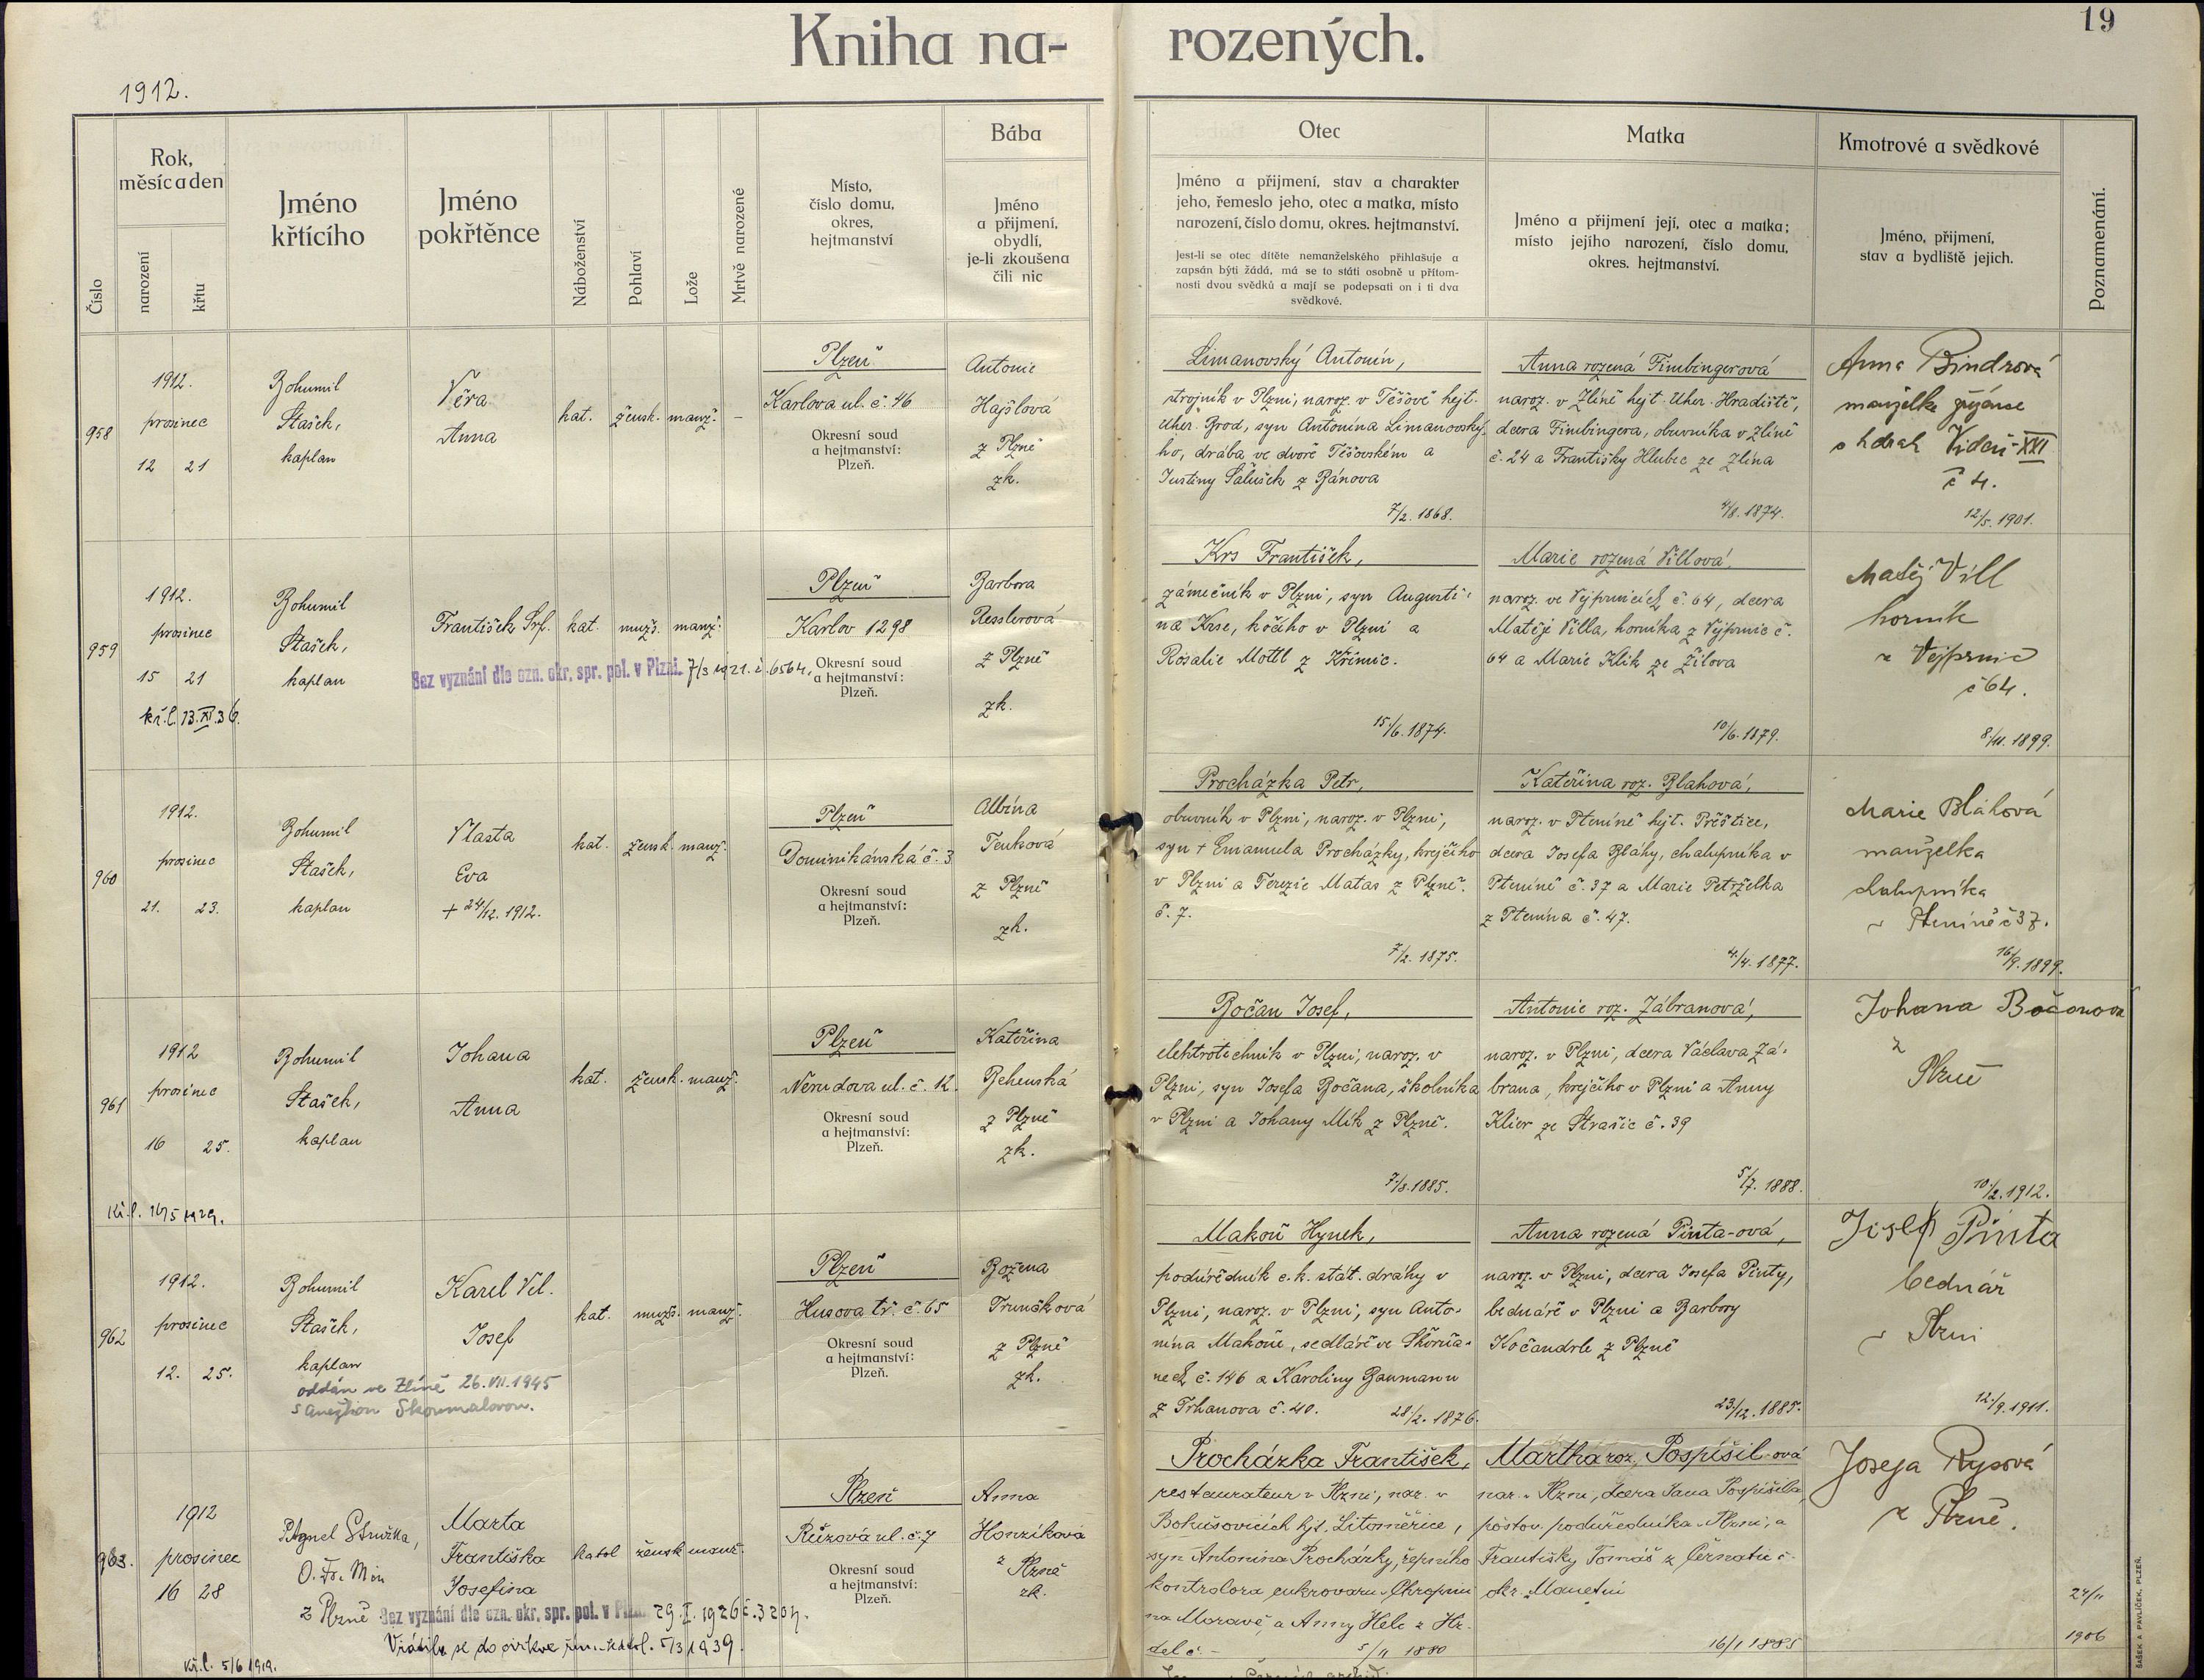
\includegraphics[scale=0.74, angle=90]{rc/matrika.eps}
\label{fig:matrika}

\section{Záznam St.B.}
\label{apx:orel}

Záznam Státní bezpečnosti o spolupráci s~Karlem Makoněm
na str. 176 plzeňského archivu bezpečnostních
složek \href{https://www.abscr.cz/data/pdf/knihy//PLA/PLA\_8.pdf}{abscr.cz/data/pdf/knihy//PLA/PLA\_8.pdf}.\\

\includegraphics[scale=0.2, angle=90]{rc/orel.png}
\label{fig:orel}

\section{Almanach Střední ekonomické školy v~Plzni}
\label{apx:almanach}

Tento almanach Střední ekonomické školy Klementa Gottwalda v~Plzni dokládá
působení Karla Makoně na této škole coby učitele.

\includepdf[pages=-]{rc/almanach.pdf}

\openright
\end{document}
